\documentclass[english,10pt,a4paper]{article}
\usepackage[T1]{fontenc}
\usepackage{geometry}
\usepackage{graphicx}
\graphicspath{{./}{../figures/wp_20260926/}{../figures/prod_20260925/}{../figures/yield_20260925/y3/}{../figures/}}
\usepackage{subcaption}
\usepackage{mathtools}
\usepackage{amssymb}
\usepackage{xcolor}
\usepackage{babel}
\usepackage{hyperref}
\usepackage{longtable}
\usepackage{tablefootnote}
\usepackage{booktabs}
\title{Roman-Rubin microlensing observation plan}
\author{Ali Salehi}
\begin{document}
	\maketitle
	
	
	\section{Introduction}
	\label{sec:intro}
	
	This white paper describes the design of a simulation of Galactic bulge microlensing observations combining the Nancy Grace Roman Space Telescope and the Vera C. Rubin Observatory. Both facilities trace back to the same source: the 2010 National Academies decadal survey, \textit{New Worlds, New Horizons in Astronomy and Astrophysics}, which ranked a wide-field infrared space telescope (what became Roman) as its top priority for a new large space mission, and a wide-field ground-based optical survey telescope (what became Rubin/LSST) as its top priority on the ground \cite{Spergel2015WFIRST,RubinAbout}. Fifteen years later, both are reaching maturity within roughly the same window, which is precisely what makes a joint observing and forecasting study like this one possible. The rest of this section summarizes each facility's mission and its relevance to microlensing, then draws the two together.
	
	\subsection{The Nancy Grace Roman Space Telescope}
	\label{subsec:roman_overview}
	
	The Nancy Grace Roman Space Telescope (Roman, formerly WFIRST) is NASA's next flagship astrophysics mission, following the James Webb Space Telescope, and is slated to launch no later than May 2027, with the project team working toward a potential launch as early as fall 2026 \cite{RomanMissionOverview}. Roman grew out of the WFIRST-AFTA Science Definition Team study \cite{Spergel2015WFIRST}, which itself merged the science cases of several earlier concepts, including a dedicated microlensing planet-finding mission. Roman carries a 2.4~m primary mirror -- the same aperture as Hubble -- feeding two instruments: the Wide Field Instrument (WFI), which performs all of the mission's survey observations, and the Coronagraph Instrument, a technology demonstration for direct exoplanet imaging that operates separately from the survey program. The WFI's 18 HgCdTe detectors give it a field of view of $0.281\,\mathrm{deg}^2$ -- about 200 times larger than Hubble's infrared channel -- across eight filters spanning $0.48$--$2.3\,\mu\mathrm{m}$; the effective area of the full WFI filter and disperser set is shown in Figure~\ref{fig:WFI}. Roman will orbit the Sun-Earth L2 point in a quasi-halo orbit, giving it a benign, stable thermal environment and an instantaneous sky-visibility annulus spanning $54^{\circ}$ to $126^{\circ}$ in solar elongation, at all ecliptic latitudes \cite{RomanMissionOverview}. The nominal mission is five years long.
	
	Roman's science program is organized around three themes -- dark energy, exoplanets, and general astrophysics -- pursued primarily through three Core Community Surveys (CCS) that will consume the majority of the primary mission's observing time \cite{ROTAC2025}: the High Latitude Wide Area Survey (HLWAS), a $\sim$1700--2000$\,\mathrm{deg}^2$ imaging and spectroscopic survey of the extragalactic sky constraining dark energy through weak lensing, baryon acoustic oscillations, and Type Ia supernovae; the High Latitude Time Domain Survey (HLTDS), which revisits one or two fields near the continuous-viewing zone every $\sim$5 days for about two years, expected to yield roughly 100,000 transient light curves in support of the same dark energy goals; and the Galactic Bulge Time Domain Survey (GBTDS), described below, which targets exoplanet demographics through microlensing.
	
	\begin{figure}
		\includegraphics[width=\linewidth]{roman_effective_area_color}
		\caption{This figure shows the effective area for the full set of Roman filters and dispersers. Source: \href{https://science.nasa.gov/mission/roman-space-telescope/wfi-technical/}{WFI Reference Information}}\label{fig:WFI}
	\end{figure}
	
	\subsubsection{The Galactic Bulge Time Domain Survey}
	\label{subsubsec:gbtds}
	
	The GBTDS's primary science driver -- identified as a high priority in the same 2010 decadal survey that recommended Roman itself -- is the demographics of cold, wide-separation exoplanets, including free-floating planets unbound to any host star, obtained through gravitational microlensing: unlike transit or radial-velocity methods, microlensing does not depend on light from the planet or its host, so it is sensitive to planets (and, more generally, any compact object, luminous or dark) regardless of whether they emit any light of their own \cite{ROTAC2025}. This is what makes microlensing simultaneously well suited to characterizing exoplanet demographics far from their host stars, and to detecting isolated stellar remnants such as neutron stars and black holes.
	
	Following the recommendations of the Roman Observations Time Allocation Committee's final report \cite{ROTAC2025}, the GBTDS will observe five contiguous $0.28\,\mathrm{deg}^2$ fields in the southern Galactic bulge plus a sixth field centered on the Galactic Center itself, for a combined footprint of about $1.7\,\mathrm{deg}^2$ -- the same field layout traced out by the footprint constants in \texttt{Bulge.h} and shown in Figure~\ref{fig:twoup_onedown} (Section~\ref{sec:locations}). Observing is concentrated into six high-cadence seasons of about 72 days each, three near the start of the mission and three near the end, timed to the spring and autumn equinoxes when the bulge is visible from L2 -- exactly the spring/autumn split shown in that same figure. During these seasons, each field is imaged roughly every 12.1 minutes in the wide F146 filter (spanning $\sim$0.93--2.00~$\mu$m, chosen to maximize photon throughput for the microlensing search) with 67-second exposures, interleaved with lower-cadence, multi-filter (F087, F213) visits every $\sim$12 hours to characterize source and lens colors. In the intervening seasons, the same fields are revisited at a sparser 3--5 day cadence to catch longer-timescale events. Using the nominal design, Roman's own predictions anticipate detecting on the order of 1400 bound exoplanets down to roughly a tenth of Earth's mass, including about 200 below three Earth masses, with sensitivity extending down to Ganymede-like masses \cite{Spergel2015WFIRST}.
	
	Every one of these numbers -- the field layout, the season structure, the F146 cadence and exposure time -- is a direct input to this project's simulation: they define the Roman half of the merged visit list described in Section~\ref{sec:input_datasets}, and the F146 filter is exactly why \texttt{Bulge.h} reserves filter index 6 alongside Rubin's six \textit{ugrizy} bands.
	
	\subsection{The Vera C. Rubin Observatory and LSST}
	\label{subsec:rubin_overview}
	
	The Vera C. Rubin Observatory, funded jointly by the NSF and DOE, sits on Cerro Pach\'on in northern Chile and houses the Simonyi Survey Telescope, an 8.4~m telescope with a novel three-mirror design that lets it slew and settle between exposures in only a few seconds \cite{RubinAbout}. Paired with the 3.2-gigapixel LSST Camera -- the largest camera ever built -- the observatory is conducting the Legacy Survey of Space and Time (LSST): a ten-year survey of the southern sky in six optical bands ($ugrizy$, spanning roughly 320--1050~nm), imaging each point on the visible sky several hundred times over the survey's lifetime \cite{Ivezic2019LSST,RubinAbout}. LSST formally began operations on 30 June 2026 and is, as of this writing, an ongoing survey. Like Roman, LSST traces back to the 2010 decadal survey, where it was the top-ranked ground-based project; its design is organized around four science pillars: probing the nature of dark energy and dark matter, taking an inventory of the Solar System, exploring the transient and variable optical sky, and mapping the structure of the Milky Way \cite{RubinAbout,Ivezic2019LSST}.
	
	\subsubsection{Microlensing with LSST}
	\label{subsubsec:lsst_microlensing}
	
	Unlike Roman, Rubin was not built around a dedicated microlensing program -- there is no LSST analog to the GBTDS. What LSST does have is depth and area: its main Wide-Fast-Deep (WFD) survey covers roughly $18{,}000\,\mathrm{deg}^2$, including parts of the Galactic plane, the bulge, and the Magellanic Clouds, at an average cadence of about once every three nights \cite{Abrams2025MicrolensingRubin}. Achieving a high microlensing discovery rate generally requires sampling at least every 2--3 days \cite{Abrams2025MicrolensingRubin}, which is finer than the WFD's default cadence but well within reach of a targeted strategy: Rubin's survey-strategy process includes a mechanism for "minisurveys" -- modest reallocations of observing time (each under about 3\% of the total survey) toward regions of particular scientific interest -- and an enhanced-cadence Galactic Plane minisurvey, motivated by more than a dozen community white papers, has been carried through detailed survey-strategy studies as one candidate implementation \cite{Street2023GalacticPlane}.
	
	Working through many such candidate cadence strategies via Rubin's own Operations Simulator, Abrams et al.\ \cite{Abrams2025MicrolensingRubin} project that LSST will discover thousands of microlensing events across the Galaxy, and find that discovery and characterization efficiency is dominated, to first order, by how much observing time is actually spent on high stellar density regions such as the bulge -- footprint choices that avoid the bulge and plane cost the survey the large majority of its microlensing yield. They further show that some \textit{rolling} cadence strategies, in which Rubin concentrates on a fraction of the sky in alternating years, can degrade microlensing parallax characterization by 15--20\% in the bulge specifically, and explicitly flag that this parallax characterization is the limiting factor in detecting free-floating black hole lenses -- events with no other observable signature.
	
	\subsection{Connecting Roman and Rubin}
	\label{subsec:connecting}
	
	Both of the papers above point toward the same conclusion from the Rubin side: cadence choices in the bulge that coincide with Roman's own high-cadence seasons would produce genuinely complementary, not merely duplicate, data. Street et al.\ \cite{Street2023GalacticPlane} note this explicitly, and Abrams et al.\ \cite{Abrams2025MicrolensingRubin} find that concentrating Rubin observations on the Roman field during Roman's observing windows could improve satellite-style parallax measurements by more than 10\%, with consequences for exoplanet, binary-star, and compact-object events alike. The physical reasoning is straightforward: Roman's six high-cadence seasons cover only about 432 of its five-year mission's $\sim$1825 days, leaving long stretches where the GBTDS alone only sparsely samples the bulge (Section~\ref{subsubsec:gbtds}); Rubin's regular, roughly three-night cadence is available throughout, including in the gaps between Roman's seasons. Ground- and space-based light curves of the same event, gathered simultaneously rather than sequentially, also give two physically independent measurements of the microlensing parallax signal from two different vantage points and instrument systematics -- the same principle satellite-parallax campaigns with Spitzer and Kepler have used before, applied here to a much closer but still independent baseline.
	
	This is precisely the synergy this project's simulation is built to quantify rather than assume. The two surveys' visit lists are carried separately and matched separately against each sightline (Section~\ref{subsec:cadence}), then interleaved into one simulated light curve in which every datum remembers which instrument produced it -- so that the combined stream is exactly what the two facilities would actually deliver, while remaining decomposable into what each contributed. And the Fisher-forecast machinery in Section~\ref{sec:fisher} is built around two separate parameter constraints for exactly this reason: a photometric one, drawing on the combined Rubin+Roman light curve to constrain the Einstein time and microlensing parallax, and an astrometric one, drawing on Roman's own high-precision centroiding to constrain the angular Einstein radius -- the same two measurements the literature identifies as necessary to break the mass-distance-velocity degeneracy and recover a lens mass at all (Section~\ref{sec:fisher}). Where the existing survey-strategy literature reasons qualitatively about whether combining Rubin and Roman helps, this project's contribution is to simulate that combination directly and report the actual, quantitative gain in event yield and parameter-recovery precision -- which is exactly the goal stated at the start of this document.
	
	\subsection{Why the Galactic bulge}
	\label{subsec:why_bulge}
	
	Four reasons, in combination, make the Galactic bulge the target of choice for this project, and for the great majority of microlensing surveys conducted since the method was first proposed.
	
	\paragraph{Stellar density.} Microlensing requires a chance alignment, to within about a milliarcsecond, between a foreground lens and a background source; both the optical depth to microlensing and the microlensing event rate consequently scale with the \emph{square} of the stellar surface density along the line of sight \cite{Terry2026HST}. Among all nearby, resolvable stellar populations, no sightline comes close to matching the bulge's surface density, which is why the bulge was the target when Paczy\'nski first proposed Galactic microlensing as an observational program \cite{Paczynski1991}.
	
	\paragraph{Distance and resolvability.} At $\sim$8~kpc, the bulge is far enough that the probability of a chance alignment is high, while its stars remain bright enough to resolve and photometer individually, from the ground and from space. This is part of why the bulge has historically been favored over the Magellanic Clouds ($\sim$50--60~kpc), which played their own historical role as a dark-matter microlensing target \cite{Paczynski1991}: at six to eight times the distance, individual Magellanic source stars are considerably fainter and harder to resolve in a crowded field for a given telescope aperture, without a corresponding gain in optical depth to compensate.
	
	\paragraph{Bulge self-lensing and the Galactic bar.} The bulge is not just a dense background of \emph{sources} -- it is also, itself, a major population of \emph{lenses}. Kiraga \& Paczy\'nski \cite{KiragaPaczynski1994} showed that a substantial fraction of bulge microlensing events are due to bulge stars lensing other bulge stars, not only foreground disk stars lensing bulge sources, which by itself increases the optical depth well beyond disk-lens-only estimates; they further showed that the remaining excess in the observed optical depth is best explained by the Galactic bar being elongated close to our line of sight, packing still more stellar mass into the same sightline. Both effects are additional to, and independent of, the surface-density argument above, and both are exactly why microlensing toward the bulge is valuable not only for exoplanet demographics but as a probe of the structure and dynamics of the Galaxy itself.
	
	\paragraph{A dedicated, comparable survey already exists.} Most importantly for this project specifically: Roman's Galactic Bulge Time Domain Survey (Section~\ref{subsubsec:gbtds}) already targets this exact region, with a well-defined field layout, cadence, and filter set \cite{ROTAC2025}. That gives this project a concrete, well-specified Roman dataset to simulate Rubin observations \emph{against}, rather than having to define a hypothetical joint survey design from scratch: the comparison this project is built around only has a sharp answer because Roman has already committed to observing this specific patch of sky.
	
	A smaller, practical point reinforces all four: the bulge's event rate does not actually peak exactly at the Galactic center. Extinction rises sharply toward $b=0^{\circ}$ even as stellar surface density also peaks there, and the two competing trends mean the observed microlensing event rate for optical/near-infrared surveys peaks a few degrees above and below the plane rather than directly on it \cite{Terry2026HST,KiragaPaczynski1994} -- which is exactly why the GBTDS fields, and this project's own footprint (Section~\ref{sec:locations}), sit at $b\approx-1.4^{\circ}$ rather than $b=0^{\circ}$.
	
	Finally, the bulge is, right now, a genuine point of convergence for several major facilities at once: alongside Roman's GBTDS, the Euclid mission has recently conducted its own Galactic Bulge Survey, and a dedicated HST program has imaged much of the same footprint specifically to support Roman's future exoplanet characterization \cite{Terry2026HST}. This project's Rubin+Roman combination sits within that same broader, current push to extract as much joint value as possible from bulge observations across facilities.
	
	\subsection{What this project sets out to do, and what it has found}
	\label{subsec:aims}

	The project asks one question in several forms: \emph{what does observing the Galactic bulge with both Roman and Rubin buy that neither buys alone?} To answer it, the simulator draws source--lens pairs along 1829 sightlines covering $67.94\,\mathrm{deg}^2$ of the bulge, generates each event's light curve and centroid track as each telescope would record them, applies one detection test three times -- to Rubin's data, to Roman's, and to both -- and forecasts each event's parameter precision with three Fisher matrices, one per survey partition (Sections~\ref{sec:montecarlo}--\ref{sec:fisher}). Every pooled number is weighted by the microlensing event rate (Section~\ref{sec:weighting}), and Section~\ref{sec:yields} turns the Monte Carlo sample into absolute event counts for any assumed abundance of the lens population. Three lens populations are simulated separately: ordinary bulge and disc stars with their remnants, isolated black holes, and neutron stars (Section~\ref{subsec:populations}).

	Four findings stand out, and the second corrects this document's own earlier headline. \textbf{(1) The Einstein radius, and with it the lens mass, is Roman's measurement}: Rubin's astrometry measures $\theta_E$ to $10\%$ for $0.1\%$ of the events Roman observes, against $50\%$ for Roman. \textbf{(2) Rubin's contribution inside Roman's footprint is narrow.} On events both surveys characterise it barely moves Roman's precision; it matters decisively only for short events that peak deep inside a gap between Roman's seasons. An earlier version of this paper reported a far larger effect; that result was produced by an inverted reddening law, now corrected (Section~\ref{subsec:reddening}). \textbf{(3) The combination still produces measurements neither survey makes alone}: $358$ footprint events are characterised only by the joint fit, and $143$ have a lens mass to $10\%$ only through it. \textbf{(4) Outside Roman's $1.5\,\mathrm{deg}^2$ footprint, Rubin is the only survey}, and $64\%$ of all detected events (event-rate weighted) lie there. The numbers behind each are in Section~\ref{sec:results}.

	\section{Input Datasets}
	\label{sec:input_datasets}
	
	This project draws on three kinds of external data, combined to turn a theoretical population of stars into a realistic, survey-specific prediction: the cadence and depth each telescope actually observes with (this section), a 3D map of interstellar reddening along each sightline (Section~\ref{sec:extinction}), and a synthetic color-magnitude diagram translating simulated stars into observed magnitudes (Section~\ref{subsec:besancon}).
	
	\subsection{Survey cadence and depth}
	\label{subsec:cadence}
	
	To be able to run observation simulations, an estimate of the actual observing conditions is needed for both telescopes -- what gets pointed where, when, in which filter, and to what depth.
	
	\subsubsection{Rubin}
	
	One great advantage of space telescopes is that they are not affected by weather and atmospheric conditions. This enables Roman to keep a constant cadence throughout each of its 72-day observation seasons. This is not the case for a ground-based telescope like Rubin, whose cadence, seeing, and depth all fluctuate with weather and scheduling. That is where operation simulations (OpSims) step in: they simulate the observing conditions for each night of the survey and produce, per simulated visit, information like cadence and seeing, which is then used in the predictions here. The results of these OpSims are published as baselines; Table~\ref{tab:opsim_columns} shows the baseline columns used in this project.
	
	
	\begin{longtable}{p{3.8cm}p{2cm}p{8.2cm}}
		\caption{Columns contained in the Rubin Observatory baseline survey simulation
			database (\texttt{baseline\_v5.3.0\_10yrs.db}). The descriptions follow the
			official Rubin Scheduler output schema unless otherwise noted.\cite{Ivezic2019LSST,Biswas2019OpSim,RubinSchedulerSchema,RubinSim}}
		\label{tab:opsim_columns}\\
		
		\toprule
		\textbf{Column} & \textbf{Units} & \textbf{Description} \\
		\midrule
		\endfirsthead
		
		\toprule
		\textbf{Column} & \textbf{Units} & \textbf{Description} \\
		\midrule
		\endhead
		
		observationId & -- &
		Unique identifier (running counter) of the simulated observation. \\&&\\
		
		\textbf{fieldRA} & deg &
		Right Ascension of the telescope boresight (ICRS). \\&&\\
		
		\textbf{fieldDec} & deg &
		Declination of the telescope boresight (ICRS). \\&&\\
		
		\textbf{observationStartMJD} & MJD &
		UTC Modified Julian Date at the beginning of the observation. \\&&\\
		
		flush\_by\_mjd & MJD &
		Time by which the queued observation is removed from scheduler consideration if not executed. \\&&\\
		
		visitExposureTime & s &
		Total on-sky exposure time of the visit. \\&&\\
		
		\textbf{band} & -- &
		Photometric bandpass used (typically $u,g,r,i,z,y$). \\&&\\
		
		filter & -- &
		Physical filter installed in the camera. Usually identical to \texttt{band}. \\&&\\
		
		rotSkyPos & deg &
		Actual orientation of the camera on the sky. \\&&\\
		
		rotSkyPos\_desired & deg &
		Desired sky rotation angle requested by the scheduler before constraints were applied. \\&&\\
		
		numExposures & -- &
		Number of exposures ("snaps") composing the visit. \\&&\\
		
		airmass & -- &
		Atmospheric airmass at the field center. \\&&\\
		
		seeingFwhm500 & arcsec &
		Atmospheric seeing FWHM referenced to 500 nm. \\&&\\
		
		\textbf{seeingFwhmEff} & arcsec &
		Effective delivered image quality used in photometric depth calculations. \\&&\\
		
		seeingFwhmGeom & arcsec &
		Geometric delivered image quality (FWHM). \\&&\\
		
		\textbf{skyBrightness} & mag arcsec$^{-2}$ &
		Predicted sky surface brightness in the observing band. \\&&\\
		
		night & -- &
		Survey night number since the start of operations. \\&&\\
		
		slewTime & s &
		Time required to slew to the field, including telescope motion, settling, readout and filter changes. \\&&\\
		
		visitTime & s &
		Total wall-clock duration of the visit. \\&&\\
		
		slewDistance & deg &
		Angular slew distance from the previous observation. \\&&\\
		
		\textbf{fiveSigmaDepth} & mag &
		Single-visit $5\sigma$ point-source limiting magnitude. \\&&\\
		
		altitude & deg &
		Altitude of the field at observation start. \\&&\\
		
		azimuth & deg &
		Azimuth of the field at observation start. \\&&\\
		
		paraAngle & deg &
		Parallactic angle (angle between celestial north and zenith). \\&&\\
		
		pseudoParaAngle & deg &
		Pseudo-parallactic angle used for camera rotation calculations. \\&&\\
		
		cloud & -- &
		Fraction of the sky covered by clouds in the weather simulation. \\&&\\
		
		moonAlt & deg &
		Altitude of the Moon. \\&&\\
		
		sunAlt & deg &
		Altitude of the Sun. \\&&\\
		
		scheduler\_note & -- &
		Scheduler label identifying the survey component or observing strategy responsible for the visit. \\&&\\
		
		target\_name & -- &
		Human-readable target name. \\&&\\
		
		target\_id & -- &
		Integer identifier of the target. \\&&\\
		
		observationStartLST & deg &
		Local Sidereal Time at the start of the observation. \\&&\\
		
		rotTelPos & deg &
		Mechanical telescope rotator angle. \\&&\\
		
		rotTelPos\_backup & deg &
		Backup rotator angle solution. \\&&\\
		
		moonAz & deg &
		Azimuth of the Moon. \\&&\\
		
		sunAz & deg &
		Azimuth of the Sun. \\&&\\
		
		sunRA & deg &
		Right Ascension of the Sun. \\&&\\
		
		sunDec & deg &
		Declination of the Sun. \\&&\\
		
		moonRA & deg &
		Right Ascension of the Moon. \\&&\\
		
		moonDec & deg &
		Declination of the Moon. \\&&\\
		
		moonDistance & deg &
		Angular separation between the field center and the Moon. \\&&\\
		
		solarElong & deg &
		Solar elongation of the field center. \\&&\\
		
		moonPhase & \% &
		Illuminated fraction of the lunar disk. \\&&\\
		
		cummTelAz & deg &
		Cumulative telescope azimuth position used internally for cable-wrap tracking. \\&&\\
		
		observation\_reason & -- &
		Reason that the observation was executed (e.g., survey, calibration, ToO). \\&&\\
		
		\textbf{science\_program} & -- &
		Science program or scheduler block associated with the observation. \\&&\\
		
		cloud\_extinction & mag &
		Photometric extinction due to clouds. \\&&\\
		
		test1 & -- &
		Reserved diagnostic field; not intended for scientific analysis. \\&&\\
		
		test2 & -- &
		Reserved diagnostic field; not intended for scientific analysis. \\&&\\
		
		\bottomrule
	\end{longtable}
	
	\subsubsection{Roman}
	
	Unlike Rubin, Roman requires no OpSim-style stochastic modeling of its cadence: from L2, weather and airmass do not apply, so the GBTDS's observing pattern is fixed by design rather than simulated. \texttt{Bulge.h} reserves filter index 6 (of \texttt{M = 7}) for F146 alongside Rubin's six \textit{ugrizy} indices, and the error functions in \texttt{helper.cpp} take any filter index generically.

	\paragraph{The schedule as actually implemented.} The survey model is built from STScI's published GBTDS design and its first-two-years schedule\footnote{\url{https://roman-docs.stsci.edu/roman-community-defined-surveys/galactic-bulge-time-domain-survey} and \url{https://roman-docs.stsci.edu/roman-community-defined-surveys/roman-observations-in-the-first-two-years-of-science-operations}} rather than from inferred arithmetic, and it differs from earlier versions of this text in three ways that matter.

	\emph{Ten seasons, not six.} The implemented schedule carries ten observing windows, six high-cadence and four low-cadence, on the five-contiguous-plus-Galactic-Center field layout.

	\emph{The mission does not start with Rubin's.} Day $0$ of the simulation clock is the earliest Rubin bulge visit, MJD $61141.312$ (2026-04-11). Roman's mission occupies days $730\rightarrow2448$ (2028-04-10 $\rightarrow$ 2032-12-23), leaving $\sim2.0$~yr of Rubin-only baseline before it and $\sim3.3$~yr after. Those Rubin-only stretches are wanted rather than wasted: they are the control arm for how much adding Roman helps, and the span over which long-$t_E$ events accumulate parallax baseline. The offset is a runtime parameter, since the real GBTDS start (2027-02-11, simulation day $306$) is expected to move; the value of $730$ used here is a deliberate choice and not an approximation of it.

	\emph{The season gaps alternate, and are not a half-year split.} An earlier model imposed a uniform $110.6$-day gap between all ten seasons, an inferred number flagged as an assumption in the generator itself. STScI's published windows show the gaps alternating between roughly $109$ and $117$ days, because Roman's sun-angle constraint sets the visibility windows rather than arithmetic. Since every gap-filling result in this paper is about what Rubin contributes \emph{between} Roman's seasons, the widths of those gaps are not a cosmetic detail.

	\emph{Two visit lists, not one.} \texttt{BulgeBaseline.dat} is not consumed as a single merged list. Each survey's epochs are matched separately and with its own field of view -- $1.75^{\circ}$ for Rubin, $\mathrm{FoV}_{\mathrm{Roman}}=0.3003^{\circ}$ for Roman -- as described in Section~\ref{sec:montecarlo}, and every light-curve datum keeps a tag saying which observatory produced it. That tag is the architectural prerequisite for everything in Section~\ref{subsec:partition}: without it, "Roman found this event" and "the combination found it" are not separable statements, and the question this paper asks cannot be answered at all. Anyone reproducing this design should put the tag in before the first light curve is generated, not retrofit it afterwards.
	
	\subsection{Extinction maps}
	\label{sec:extinction}
	
	Interstellar dust reddens and dims every star in the simulated catalog, and getting this reddening right is what separates a physically meaningful yield prediction from an aspirational one. Toward the Galactic bulge this matters more than almost anywhere else on the sky: the sightline studied here, $(l,b)=(0.5^{\circ},-1.4^{\circ})$, sits only about $1.4^{\circ}$ from the Galactic plane, where dust reddening is both extremely high and extremely patchy on scales of arcminutes. A single, sightline-averaged extinction value is not an adequate description of a $0.1\,\mathrm{deg}^2$ field, let alone the full multi-tile footprint shown in Figure~\ref{fig:twoup_onedown}.
	
	Two separate extinction estimates appear in this project, and how they are kept from double-counting is explained in Section~\ref{sec:extinction-fix}:
	
	\begin{enumerate}
		\item \textbf{The Besan\c{c}on model's own, built-in extinction}, applied internally while the synthetic stellar catalog is generated.
		\item \textbf{A custom 3D dust map}, built separately from public survey data and applied in the C++ simulation at each star's actual simulated position.
	\end{enumerate}
	
	\subsubsection{Besan\c{c}on's built-in extinction options}
	
	The Besan\c{c}on model offers three ways of assigning extinction to a simulated star \cite{Robin2003Besancon}:
	
	\begin{enumerate}
		\item \textit{Diffuse extinction by a dusty disk} -- a smooth interstellar layer, with density following the same Einasto profile used for the thin disc, normalized to a single mean absorption rate (in V) at the solar neighbourhood. This project's model run used this option, at the tool's recommended default of $0.7$~mag/kpc for intermediate/high-latitude fields (adjustable).
		\item \textit{Diffuse extinction with discrete clouds} -- the same diffuse layer, with individually placed high-density cloud clumps superimposed.
		\item \textit{The Marshall et al. extinction model} -- a genuine 3D extinction map built by comparing observed 2MASS photometry against the Besan\c{c}on model's own predicted intrinsic colors, valid for $-100^{\circ}<l<100^{\circ}$, $-10^{\circ}<b<10^{\circ}$ \cite{Marshall2006Extinction}, falling back to the diffuse-disk law outside that range.
	\end{enumerate}
	
	Option 1 is a reasonable default far from the plane, where dust really is diffuse and roughly uniform. At $b=-1.4^{\circ}$, however, a uniform $0.7$~mag/kpc law is almost certainly a substantial underestimate of the true, highly structured extinction toward the bulge -- which is precisely why this project builds its own 3D map rather than relying on it for the final photometry. Rather than switching the Besan\c{c}on \emph{query} itself to Option 3, this project sidesteps the choice entirely by running the query with diffuse extinction set to zero (Section~\ref{sec:extinction-fix}), leaving the custom map as the sole source of reddening.
	
	\subsubsection{A custom 3D map from public dust surveys}
	
	The project's own extinction map is generated by \texttt{maps2.py}, using the \texttt{dustmaps} package \cite{Green2018Dustmaps}. For each sightline, extinction is evaluated on an evenly spaced distance grid out to \texttt{MaxD}~$=20$~kpc, drawing on two different underlying surveys depending on declination:
	
	\begin{itemize}
		\item \textbf{Bayestar19} \cite{Green2019Bayestar}, for declinations north of $-30^{\circ}$: a 3D dust map built from Gaia parallaxes and Pan-STARRS1/2MASS photometry of nearby stars.
		\item \textbf{The Zucker et al. (2025) DECaPS 3D dust map} \cite{Zucker2025DECaPS}, for declinations south of $-30^{\circ}$: built from the deeper DECaPS2 photometric survey, covering the southern Galactic plane ($239^{\circ}<l<6^{\circ}$, $|b|<10^{\circ}$) that Bayestar19 does not reach.
	\end{itemize}
	
	This branch matters concretely for this project: computing the declinations of the published Roman GBTDS field pointings places them at approximately $-28^{\circ}$ to $-30^{\circ}$, straddling the Bayestar/DECaPS boundary closely rather than sitting cleanly on one side, so a per-sightline branch is necessary rather than picking one map for the whole survey footprint.
	
	Bayestar19 reports reddening in an internal, arbitrary unit rather than $E(B\!-\!V)$ directly; \texttt{maps2.py} converts it via the commonly used $\times 0.884$ scale factor. The DECaPS map reports $E(B\!-\!V)$ directly. Both are then converted to $A_V$ assuming $R_V=3.1$.
	
	\paragraph{Known issue to fix.} The \texttt{dustmaps} documentation specifies $R_V=3.32$, not $3.1$, for converting the DECaPS map's $E(B\!-\!V)$ to $A_V$ \cite{DustmapsDocs}. \texttt{maps2.py} currently uses $3.1$ for both maps uniformly -- worth correcting for the DECaPS branch specifically before the extinction files are regenerated.
	
	\paragraph{Open item: reconciling sightline files.} \texttt{maps2.py} writes one output file per sightline (\texttt{bayestar\_\{l\}\_\{b\}.txt}), while the C++ simulation (\texttt{Bulge\_LSST.cpp}) reads a single combined file, \texttt{Marshalmap.txt}. Either a concatenation step exists outside the files reviewed here, or this needs to be added. Relatedly, \texttt{maps2.py} draws its sightline list from every row of \texttt{BulgeBaseline.dat}, which is a per-\emph{visit} file; the same field pointing is revisited many times over a 10-year baseline, so the sightline list should likely be deduplicated on $(l,b)$ before generating extinction files, to avoid redundant identical sightlines.
	
	\paragraph{A structural note.} The sightlines used for the extinction map are read directly from \texttt{BulgeBaseline.dat} -- i.e., extinction is mapped exactly where the survey will actually point, rather than on an independently chosen grid. This is a genuine, load-bearing link between two of this project's three core datasets, not just a downstream convenience.
	
	\subsubsection{Reconciling Besan\c{c}on's extinction with the custom map}
	\label{sec:extinction-fix}
	
	The double-extinction risk described above is avoided by construction: the Besan\c{c}on catalog used in this project (\texttt{bos7.dat}) is generated with diffuse extinction (Section~\ref{sec:extinction}) set to zero, rather than the tool's recommended $0.7$~mag/kpc default. Every native Besan\c{c}on magnitude, and \texttt{Mbol} in particular, is therefore already intrinsic, and the catalog's own \texttt{Av} column is uniformly zero -- so passing it directly into the MIST bolometric-correction interpolation (Section~\ref{subsec:interpolation}) has no effect, and every filter magnitude \texttt{interpolate2.py} writes out is already a true, unreddened absolute magnitude. \texttt{Mab[i]} then flows into \texttt{Map[i]} in \texttt{Lensing.cpp} as an absolute magnitude plus distance modulus plus exactly one extinction term (\texttt{Ai[i]}, from the custom 3D map at the star's simulated distance) -- the single-reddening structure this pipeline is intended to have.
	
	This choice also disposes of a query-time selection effect: Besan\c{c}on's own apparent-magnitude window ($10<V<29$) is now evaluated at zero extinction, which is the most permissive assumption possible at the faint end -- no star that would fall within the survey's true magnitude range under any realistic (larger) extinction is excluded by this cut, since real reddening can only push a star fainter, never brighter, relative to the zero-extinction case used for selection. A residual, likely negligible edge case remains at the bright end: a star intrinsically brighter than $V=10$ could in principle be excluded here even though real extinction would have pushed it fainter into range; given this project's sources of interest span $15$--$26$~mag (Section~\ref{subsec:besancon}), this is not expected to matter in practice.
	
	\subsubsection{From $A_V$ to every band: the reddening law, and a bug that inverted it}
	\label{subsec:reddening}

	The 3D map supplies $A_V$ at the source's simulated distance, interpolated along the nearest extinction sightline. Each band's extinction is then
	\begin{equation}
		A_i \;=\; A_V\,\frac{A_{\lambda_i}}{A_V}(R_V) \;+\; \epsilon_i, \qquad \epsilon_i \sim \mathcal{N}(0,\sigma_i)\ \text{truncated at}\ \pm\sigma_i, \qquad A_i \to \max(A_i, 0),
	\end{equation}
	and the apparent magnitude is $m_i = M_i + 5\log_{10}(100\,D_s/\mathrm{kpc}) + A_i$. The small per-band scatter $\sigma_i = (0.022, 0.020, 0.017, 0.017, 0.027, 0.027, 0.04)$~mag for $ugrizy$ and F146 stands in for sub-sightline patchiness; the F146 value is a K-band placeholder. The extinction ratio follows \cite{Cardelli1989},
	\begin{equation}
		\frac{A_\lambda}{A_V} = a(x) + \frac{b(x)}{R_V}, \qquad x \equiv \frac{1}{\lambda/\mu\mathrm{m}},
	\end{equation}
	with, in the infrared ($0.3 \le x < 1.1$), $a = 0.574\,x^{1.61}$ and $b = -0.527\,x^{1.61}$, and in the optical ($1.1 \le x < 3.3$, $y = x - 1.82$)
	\begin{align*}
		a &= 1 + 0.17699y - 0.50447y^2 - 0.02427y^3 + 0.72085y^4 + 0.01979y^5 - 0.77530y^6 + 0.32999y^7,\\
		b &= 1.41338y + 2.28305y^2 + 1.07233y^3 - 5.38434y^4 - 0.62251y^5 + 5.30260y^6 - 2.09002y^7 .
	\end{align*}
	$R_V$ depends on the Galactic component the source belongs to: $2.5$ for the bulge, following the low bulge values measured toward the inner Galaxy, and $3.1$ for the thin disc, thick disc and halo. The seven effective wavelengths are $0.367, 0.482, 0.622, 0.755, 0.869, 0.971$ and $1.464\,\mu$m, which give, at the bulge's $R_V=2.5$,

	\begin{center}
	\begin{tabular}{lccccccc}
		\toprule
		band & $u$ & $g$ & $r$ & $i$ & $z$ & $y$ & F146 \\
		\midrule
		$A_\lambda/A_V$, correct & 1.694 & 1.216 & 0.854 & 0.627 & 0.460 & 0.381 & 0.197 \\
		$A_\lambda/A_V$, as run before 2026-09-22 & 0.072 & & & & & & 0.751 \\
		\bottomrule
	\end{tabular}
	\end{center}

	\paragraph{The inversion.} Until 2026-09-22 the code computed $x = 1/\lambda$ and passed $x$ to functions that themselves take a wavelength and invert it again, so the law was evaluated at wavenumber $=\lambda$. The result was not noise but a mirror image: extinction \emph{rose} from blue to red, from $0.07$ in $u$ to $0.75$ in F146, where it should fall from $1.69$ to $0.20$. At the median $A_V \approx 3.8$ of detected events, Rubin's $r$-band sources were $\sim\!3.7$~mag too bright and Roman's F146 sources $\sim\!3$~mag too faint -- in opposite directions for the two telescopes, and therefore directly in the quantity this project exists to measure. It was found not by a test but by looking: a sightline flagged as unusually rich in Rubin-only events turned out to carry sources with $F146 \approx 28$--$29$ against $r \approx 19.5$, which a reddened bulge star cannot have. The fix passes the wavelength straight through, and a unit test with no data dependencies (\texttt{make extinctiontest}) pins $A_V/A_V = 1$ at $V$ for $R_V=2.5$ and $3.1$, a monotone fall from $u$ to F146, and all seven band values above against an independent evaluation of CCM89 to $5\times10^{-3}$; run against the old code, it fails. Every result in this document from Section~\ref{sec:results} onward comes from runs made after the fix, and Section~\ref{subsec:fixeffect} measures what it changed.

	\paragraph{A lesson for anyone reimplementing this.} A reddening law has two properties that can be checked without any data: $A_\lambda/A_V = 1$ at $V$, and $A_\lambda$ falls monotonically with wavelength from the ultraviolet to the near-infrared. The inverted law fails both -- it gives $A_V/A_V \approx 0.14$ at $V$ -- and was in production for two months because neither had been written down. Both cost nothing and belong in any pipeline that applies extinction per band.

	\subsection{Color maps}

	A color-magnitude diagram (CMD), in the sense used throughout this project, is the bridge between theoretical stellar population synthesis and the actual observables a survey records. The Besan\c{c}on model (Section~\ref{subsec:besancon}) supplies the physical population of stars along a given sightline -- their masses, ages, temperatures, and evolutionary state -- but not, in this pipeline, their photometry in Rubin or Roman's own filters. MIST's bolometric correction tables (Section~\ref{subsec:mist}) supply the translation from those intrinsic stellar parameters into specific instrumental bandpasses. \texttt{interpolate2.py} (Section~\ref{subsec:interpolation}) is the numerical machinery that carries out that translation, star by star, producing the synthetic Rubin+Roman photometry that the C++ simulation treats as its library of possible source and lens types.
	
	\subsubsection{The Besan\c{c}on Galaxy Model}
	\label{subsec:besancon}
	
	The Besan\c{c}on model is a semi-empirical stellar population synthesis model of the Milky Way \cite{Robin2003Besancon}. For an assumed scenario of Galactic formation and evolution, it simulates the stellar content of the Galaxy across four populations -- thin disc, thick disc, bulge, and stellar halo/spheroid -- returning, for each simulated star, its mass, age, effective temperature, surface gravity, metallicity, population membership, distance, and (subject to the extinction option chosen; Section~\ref{sec:extinction}) its native photometry.
	
	\paragraph{Query configuration for this project}
	
	The catalog used in this project (\texttt{bos7.dat}) was generated for a single pencil-beam sightline at $(l,b)=(0.5^{\circ},-1.4^{\circ})$, covering $0$--$8$~kpc in distance over a solid angle of $0.1\,\mathrm{deg}^2$ -- matching \texttt{DBulge = 8} in \texttt{Bulge.h}. The relevant model parameters, taken directly from the run header, are:
	
	\begin{itemize}
		\item \textbf{Initial mass function:} a broken power law, shallow ($\propto M^{-0.6}$) below $1\,M_\odot$ across three sub-bins, steepening to a Salpeter-like $\propto M^{-2}$ above $1\,M_\odot$.
		\item \textbf{Star formation history:} constant star-formation rate for the disc ($\nu=0.4$).
		\item \textbf{Density laws:} an Einasto thin disc, a flared, warped bar/bulge, a two-episode $\mathrm{sech}^2$ thick disc, and a Hernquist spheroid.
		\item \textbf{Atmosphere models:} Basel 3.1, with $R_V=3.1$ -- matching the $R_V$ assumed by the MIST bolometric-correction grid (Section~\ref{subsec:mist}).
		\item \textbf{Kinematics: explicitly disabled} in this run (\texttt{No kinematics} in the header). This is the reason \texttt{vrel()} exists in \texttt{Lensing.cpp} at all: source and lens velocities are not supplied by Besan\c{c}on, but synthesized independently from population-dependent velocity-dispersion draws ($\sigma_R,\sigma_T,\sigma_Z$ per component) plus solar reflex motion.
		\item \textbf{Apparent-magnitude selection:} $10<V<29$ -- evaluated at zero extinction for this project's catalog (Section~\ref{sec:extinction-fix}).
	\end{itemize}
	
	\paragraph{Population codes}
	
	The catalog's \texttt{Pop} column identifies which of eleven sub-populations a star belongs to. The mapping below is read directly off the run header's metallicity table, and lines up exactly with the grouping used in \texttt{interpolate2.py} (thin disc: \texttt{Pop} 1--7; thick disc: \texttt{Pop} 8 and 11; halo: \texttt{Pop} 9; bulge: \texttt{Pop} 10), consistent with the seven-age-subcomponent division of the thin disc described in \cite{Robin2003Besancon}.
	
	\begin{table}[htbp]
		\centering
		\begin{tabular}{clcc}
			\toprule
			\textbf{Pop} & \textbf{Component} & \textbf{Age (Gyr)} & \textbf{$\langle\mathrm{[M/H]}\rangle$} \\
			\midrule
			1  & Thin disc            & 0.15 & $+0.01$ \\
			2  & Thin disc            & 1    & $\phantom{+}0.00$ \\
			3  & Thin disc            & 2    & $-0.02$ \\
			4  & Thin disc            & 3    & $-0.03$ \\
			5  & Thin disc            & 5    & $-0.05$ \\
			6  & Thin disc            & 7    & $-0.09$ \\
			7  & Thin disc            & 10   & $-0.12$ \\
			8  & Thick disc (young)   & --   & $-0.47$ \\
			9  & Halo (spheroid)      & --   & $-1.48$ \\
			10 & Bulge (bar)          & --   & $\phantom{+}0.00$ \\
			11 & Thick disc (old)     & --   & $-0.78$ \\
			\bottomrule
		\end{tabular}
		\caption{Population codes in the Besan\c{c}on output, reconstructed from the model run header's metallicity table. Ages for the thick disc, halo, and bulge sub-populations are not single-valued in the model and are omitted here.}
		\label{tab:pop_codes}
	\end{table}
	
	\paragraph{Columns used downstream}
	
	Of the columns the model returns, this pipeline uses \texttt{Teff}, \texttt{logg}, \texttt{Mass}, \texttt{Age}, \texttt{Mbol}, \texttt{[M/H]}, \texttt{[a/Fe]}, \texttt{Av}, \texttt{Dist}, and \texttt{Pop}. The model's own native photometry (V, B, U, R, I, J, H, K, and their colors) is not used -- Rubin and Roman magnitudes are computed independently via the MIST bolometric-correction tables instead (Section~\ref{subsec:mist}), which is also why the model's kinematics being disabled has no further consequence beyond the velocities themselves.
	
	\subsubsection{MIST bolometric correction tables}
	\label{subsec:mist}
	
	The MIST project provides theoretical stellar evolutionary tracks and isochrones computed with the MESA stellar evolution code \cite{Choi2016MIST}, and, alongside them, precomputed bolometric correction (BC) tables: grids of $\mathrm{BC}(T_{\mathrm{eff}}, \log g, A_V, \mathrm{[Fe/H]}, \mathrm{[\alpha/Fe]})$ for a range of photometric systems, spanning $A_V=0$ to $6$ at $R_V=3.1$. This project uses the v2 tables for both the Rubin/LSST $ugrizy$ system and the Roman WFI filter set (including F146).
	
	A bolometric correction converts a star's bolometric magnitude into its apparent magnitude in one specific filter:
	\[
	m_{\mathrm{filter}} = M_{\mathrm{bol}} - \mathrm{BC}_{\mathrm{filter}}(T_{\mathrm{eff}}, \log g, A_V, \mathrm{[Fe/H]}, \mathrm{[\alpha/Fe]})
	\]
	This is the mechanism that turns Besan\c{c}on's intrinsic stellar parameters into the specific, instrument-dependent magnitudes the survey simulation needs. Because $A_V$ is one of the grid's five axes, the same BC table could, in principle, also supply extinction -- but for this project's catalog that axis is uniformly zero already (Section~\ref{sec:extinction-fix}), so reddening is supplied solely by the project's own 3D map rather than by the BC table's own $A_V$ dimension.
	
	\subsubsection{Interpolation: from catalog to synthetic photometry}
	\label{subsec:interpolation}
	
	\texttt{interpolate2.py} is the code that carries out the translation described above, for every star in the Besan\c{c}on catalog. Its steps are:
	
	\begin{enumerate}
		\item \textbf{Metallicity conversion.} Besan\c{c}on reports \texttt{[M/H]} and \texttt{[a/Fe]} separately; MIST's grid is indexed by \texttt{[Fe/H]} and \texttt{[a/Fe]}. The two are related by the standard alpha-enhanced metallicity relation, $\mathrm{[Fe/H]} = \mathrm{[M/H]} - \log_{10}\!\left(0.638\times10^{\mathrm{[a/Fe]}} + 0.362\right)$.
		\item \textbf{Grid construction.} The MIST BC table (all files in the relevant \texttt{Rubin} or \texttt{Roman} directory) is loaded, and a five-dimensional \texttt{RegularGridInterpolator} is built over $(\log T_{\mathrm{eff}}, \log g, A_V, \mathrm{[Fe/H]}, \mathrm{[\alpha/Fe]})$.
		\item \textbf{Per-star interpolation.} For every filter in the chosen photometric system, each star's parameters are evaluated against the grid and combined with \texttt{Mbol} to give an apparent magnitude, as in Section~\ref{subsec:mist}. Stars whose parameters fall outside the grid's coverage (extreme temperature, metallicity, or -- currently -- $A_V$) come back as \texttt{NaN} and are dropped.
		\item \textbf{Assembly.} The Rubin and Roman filter sets are computed in two passes over the same underlying catalog and combined, then split by galactic component (thin disc / thick disc / halo / bulge, using the \texttt{Pop} mapping in Table~\ref{tab:pop_codes}) into the per-component files (\texttt{thin\_disk.dat}, \texttt{bulge.dat}, etc.) that the C++ simulation reads as \texttt{cm.Mab\_thin}, \texttt{cm.Mab\_bulge}, and so on.
	\end{enumerate}
	
	One coverage caveat worth quantifying rather than assuming away: the MIST v2 grid's $\mathrm{[\alpha/Fe]}$ axis appears to extend only to $+0.6$, while the Besan\c{c}on run allowed $\mathrm{[\alpha/Fe]}$ up to $+0.70$ (Section~\ref{subsec:besancon}). Some genuine fraction of alpha-enhanced stars will therefore be silently dropped as \texttt{NaN}; the diagnostic print statement already present in \texttt{read\_input()} (\texttt{aFe > 0.6}) reports exactly this count and is worth citing directly as a completeness caveat in the methods section, rather than leaving it as an unreported side effect.
	
	For why the $A_V$ axis is kept at zero for this project's catalog, see Section~\ref{sec:extinction-fix}.
	
	\section{Locations}
	\label{sec:locations}
	
	\begin{figure}[htbp]
		\centering
		
		% Top row
		\begin{subfigure}{0.48\textwidth}
			\centering
			\includegraphics[width=\linewidth]{roman_967_spring_aladinX}
			\caption{Locations of Spring surveys}
			\label{fig:a}
		\end{subfigure}
		\hfill
		\begin{subfigure}{0.48\textwidth}
			\centering
			\includegraphics[width=\linewidth]{roman_967_autumn_aladinX}
			\caption{Locations of Autumn surveys}
			\label{fig:b}
		\end{subfigure}
		
		\vspace{0.5cm}
		
		% Bottom row
		\begin{subfigure}{0.48\textwidth}
			\centering
			\includegraphics[width=\linewidth]{roman_967_both_aladinX}
			\caption{Both locations combined}
			\label{fig:c}
		\end{subfigure}
		
		\caption{A Galactic coordinate grid is shown (green), which shows that the mid-line of the five contiguous tiles are at the desired galactic coordinates (0.5, -1.4), and there is one non-contiguous tile at the Galactic Center.}
		\label{fig:twoup_onedown}
	\end{figure}
	
	\section{Observational Error Models}
	\label{sec:error_models}
	
	Every simulated measurement in this project carries one of two fundamentally different kinds of uncertainty. \textbf{Photometric error} is the uncertainty on a star's measured brightness, and to first order depends only on how many photons were collected relative to the noise (sky background, detector read noise, Poisson statistics on the source itself) -- it does not depend strongly on how sharply focused the image is. \textbf{Astrometric error} is the uncertainty on a star's measured \emph{position}, and depends on both the photon budget \emph{and} the width of the point-spread function (PSF): a star's centroid can, in principle, be measured far more precisely than the PSF's own width would naively suggest, because that precision comes from how the collected light is distributed across the PSF, not from resolving the PSF itself. For a wide range of realistic PSF shapes, the achievable 1$\sigma$ centroiding precision scales as
	\[
	\sigma_{\mathrm{ast}} \approx 0.7\,\frac{\mathrm{FWHM}}{\mathrm{S/N}},
	\]
	a relation established for exactly this kind of crowded, bulge-field astrometry \cite{KuijkenRich2002}, and shown to be close to the fundamental Cram\'er-Rao information limit for standard centroiding estimators \cite{VakiliHogg2016}. This is the reason a sharper PSF (space-based Roman, Section~\ref{subsec:roman_errors}) buys astrometric precision so much more efficiently than a wider, seeing-limited one (ground-based Rubin, Section~\ref{subsec:rubin_errors}), even when the two instruments collect comparable numbers of photons.
	
	\subsection{Rubin}
	\label{subsec:rubin_errors}
	
	Photometric error (\texttt{errlsstM}) follows the standard random-photometric-error model adopted for LSST's own survey design \cite{Ivezic2019LSST}:
	\[
	\sigma_{\mathrm{phot}}^2 = \delta^2 + \left[(0.04-\gamma)\,x + \gamma\,x^2\right], \qquad x \equiv 10^{0.4(m-m_5)},
	\]
	where $m_5$ is that visit's actual $5\sigma$ depth (Table~\ref{tab:opsim_columns}), $\gamma$ is a band-dependent constant controlling where the error transitions from source-photon-dominated to sky-background-dominated, and $\delta=0.005$ is a fixed photometric systematic floor. Astrometric error (\texttt{errlsstA}) is instead a direct lookup against a digitized empirical precision-vs-magnitude curve for LSST, rather than an evaluation of the FWHM/SNR relation above -- a reasonable simplification given that ground-based seeing genuinely varies visit to visit (the per-band \texttt{FWHM} entries in \texttt{Bulge.h}, $\sim$0.9--1.2 arcsec, are typical, seeing-limited values, roughly ten times wider than Roman's diffraction-limited PSF; Section~\ref{subsec:roman_errors}), but it does mean this project's Rubin astrometric errors reflect a single representative seeing curve rather than the actual per-visit conditions already available elsewhere in the pipeline (Table~\ref{tab:opsim_columns}).
	
	\subsection{Roman}
	\label{subsec:roman_errors}
	
	Roman's WFI delivers a far sharper and far more stable PSF than any ground-based instrument: its F146 point-spread function has a FWHM of roughly 90--105~mas \cite{Fardeen2024PBH,ROTAC2025} against a 110~mas pixel scale, compared with Rubin's seeing-limited $\sim$0.9~arcsec, with no night-to-night atmospheric variation to average over. This is why the $\theta_E$ measurement the Fisher forecast (Section~\ref{sec:fisher}) depends on is Roman's, and only Roman's.
	
	\paragraph{Astrometric error (\texttt{errRomanA}).} Roman's per-exposure centroiding precision is evaluated from the source's own F146 magnitude, in three regimes:
	\[
	\sigma_{\mathrm{ast}}(m) = \begin{cases}
	1.1~\mathrm{mas} & m \le 20.62\\
	1.1\times10^{0.333\,(m-20.62)}~\mathrm{mas} & 20.62 < m \le 23.5\\
	10\times10^{0.4\,(m-23.5)}~\mathrm{mas} & m > 23.5.
	\end{cases}
	\]
	The floor is $1\%$ of the pixel, a centroiding systematic rather than photon noise, which is why it does not improve for brighter sources \cite{Sanderson2019WFIRSTastrometry}. The two anchors and the $23.5$~mag background transition are taken from a Roman black-hole astrometric-binary study \cite{RomanBHbinaries}, whose curve derives from Pandeia and the Roman astrometry simulation tool; the $0.333$/mag slope between them is fixed by those anchors, and sits between the $0.2$/mag of pure source-photon noise and the $0.4$/mag of pure background domination because the transition is already under way across that range.
	
	\textbf{Two factors of ten are easy to get wrong here, and both are fatal to the astrometric result.} The first is that the widely quoted $0.1$~mas Roman astrometric precision is a \emph{daily-binned} number, roughly $100$ exposures stacked; the per-epoch error this simulation needs is the single-exposure value, because one row of the Roman visit list is one $66$-second exposure at a $12.1$-minute cadence. Using $0.1$~mas as a per-epoch error would overstate Roman's astrometry tenfold and flatter every $\theta_E$ and lens-mass forecast in the study. The second is that $1.1$~mas is the \emph{bright-source} floor and does not describe a GBTDS microlensing source: those are faint bulge main-sequence stars, median $F146\approx21.8$ among the Roman-observed detections (event-rate weighted), for which the same curve gives $2.75$~mas. (Before the reddening law was corrected, Section~\ref{subsec:reddening}, the F146 sources were $\sim\!1$~mag too faint in this sample -- median $23.0$ -- and the curve gave $6.69$~mas.) Evaluating the error at each source's own magnitude, rather than quoting the floor, changes the astrometric conclusion by a factor of $2.5$.
	
	\paragraph{Photometric error (\texttt{errRomanM}).} Roman's photometric error is a lookup against a tabulated magnitude--error curve rather than an evaluation of the Rubin formula above. This is the right shape of model for a space-based survey -- there is no per-visit $5\sigma$ depth to interpolate against, because there is no atmosphere to vary -- but the present implementation takes the nearest tabulated magnitude rather than interpolating between entries, which is a placeholder and is recorded as such in Section~\ref{sec:openitems}. Wilson et al.\ \cite{Wilson2023GBTDS} derive a pixel-level F146 noise model directly from simulated GBTDS images, identifying $F146\approx22$ as the source-to-background transition; that is the model a replacement should be built from.
	
	\section{Monte Carlo Simulation}
	\label{sec:montecarlo}
	
	For each field pointing (Section~\ref{sec:locations}), the simulation estimates a detection efficiency, an expected event rate, and -- via the Fisher forecast (Section~\ref{sec:fisher}) -- a parameter-recovery precision, by repeatedly drawing a random source and a random lens along the sightline, generating the light curve and astrometric trajectory that the combined Roman+Rubin observations would actually record, and testing whether that simulated data stream would be flagged as a detected microlensing event. This simulate-detect-forecast structure follows the same general approach used to produce Roman's own exoplanet-yield predictions \cite{penny2019predictions}, applied here to the combined Roman+Rubin case rather than Roman alone.
	
	\subsection{Field-by-field scan}
	
	For each $(l,b)$ pointing in the footprint (Section~\ref{sec:locations}), the code collects the observations that actually cover that pointing. The two surveys are handled \emph{separately} rather than through a single merged visit list, because they have different fields of view and different schedules: Rubin's is matched within a radius $\mathrm{FoV}=1.75^{\circ}$, Roman's within $\mathrm{FoV}_{\mathrm{Roman}}=0.3003^{\circ}$. Each call returns its own epoch count and its own minimum gap between consecutive visits (\texttt{minc}), and it is the finer of the two that sets the time resolution the simulated light curve must sample. Keeping them separate is not bookkeeping: a sightline can sit inside Roman's footprint or outside it, and the two cases differ by roughly $5\times10^{4}$ epochs, which is the single largest factor controlling what the joint fit can do at that position.

	The epoch matcher also removes duplicate timestamps. Two visits can legitimately carry the same recorded time for one sky position when the circles of two adjacent pointings overlap and the pointings share an observing schedule -- which is exactly the situation between neighbouring Roman fields, whose $0.3003^{\circ}$ radius exceeds half the $\sim0.41^{\circ}$ field spacing. There is no meaningful cadence between two simultaneous visits, so the first is kept and the duplicate skipped. The occurrence is logged rather than silently absorbed: occasional firing near field boundaries is expected, but constant firing would indicate a sorting or data problem in the baseline file that must be fixed at source instead of papered over here.

	\texttt{Disk\_model} then evaluates the stellar density laws at that pointing (Section~\ref{subsec:besancon}), and \texttt{nearestSightline} identifies the closest extinction sightline (Section~\ref{sec:extinction}) to use for that field. A sightline that neither survey visits is skipped outright: with no epochs, no light curve can carry a datum, no event can be detected, and the per-field stopping criterion below could never be satisfied.
	
	\subsection{Stratified sampling of the sky}
	\label{subsec:stratification}

	Roman's GBTDS footprint is a small fraction of the scanned region, so a scan on a uniform grid spends almost all of its draws where the joint Fisher matrix is simply Rubin's, and the events that actually test the combination stay rare no matter how long the run continues. The scan is therefore stratified in sky position: sightlines inside the footprint are visited on a fine grid, sightlines outside on a coarse one. The production runs reported here use $0.1^{\circ}$ inside and $0.2^{\circ}$ outside, giving $147$ footprint sightlines and $1{,}682$ outside, covering $67.94$~deg$^2$ in total.

	The sample is then deliberately \emph{not} proportional to sky area, so every event row carries $w_{\mathrm{area}}$, the solid angle in deg$^2$ that its sightline stands for. Anything pooled across the scan -- a survey-wide yield, a histogram over all detections -- must be weighted by it, or it describes a sky in which Roman covers whatever fraction of the \emph{sample} the stratification bought rather than the fraction of the \emph{sky} it actually covers. Quantities computed at a single sightline, restricted to the footprint, or formed as a per-event ratio are unaffected, because the sightline a draw came from is not an input to them.

	\subsection{Event generation and pre-selection}
	
	\paragraph{Lens populations.}\label{subsec:populations} The lens mass function is a run-time choice (\texttt{-{}-population}), and three populations are simulated, each in its own run with its own output files. This is worth stating as a first-class modelling choice rather than a detail, because it propagates into every quantity the study reports and it is the easiest thing in the pipeline to get silently wrong: a mass range borrowed from a MACHO dark-matter search ($3$--$5000\,M_\odot$) produces a median lens mass of $387\,M_\odot$, a median Einstein crossing time of $953$~d and a median angular Einstein radius of $13.75$~mas, against a bulge whose median lens is a few tenths of a solar mass and whose typical event lasts tens of days. Those four medians are a cheap and decisive sanity check on any reimplementation: if they do not look like a bulge, nothing downstream describes one either.

	\emph{Ordinary lenses} (\texttt{bulge}, the default) are the present-day population of a $\sim\!10$~Gyr-old bulge. An \emph{initial} mass is drawn from the Kroupa (2001) broken power law \cite{Kroupa2001}, $\mathrm{d}N/\mathrm{d}M = k_i M^{-\alpha_i}$ with $\alpha = 0.3, 1.3, 2.3$ on $[0.01, 0.08]$, $[0.08, 0.5]$ and $[0.5, 120]\,M_\odot$, and the $k_i$ fixed by continuity at the breaks, $k_2 = k_1\,0.08^{\alpha_2-\alpha_1}$ and $k_3 = k_2\,0.5^{\alpha_3-\alpha_2}$ -- a discontinuous IMF would put steps in the mass, and therefore the $t_E$, distribution. It is sampled by inverse CDF: a segment is chosen in proportion to its star count $k_i\int M^{-\alpha_i}\mathrm{d}M$, then that segment's CDF is inverted, one uniform draw each. The initial mass is then mapped to whatever still exists to act as a lens: below the $1\,M_\odot$ turnoff the star is unevolved and lenses at its birth mass; $1$--$8\,M_\odot$ leaves a white dwarf of $0.109\,M_i + 0.394\,M_\odot$ (the semi-empirical initial--final relation of Kalirai et al.\ 2008); $8$--$20\,M_\odot$ leaves a $1.4\,M_\odot$ neutron star; above $20\,M_\odot$, a black hole of $0.24\,M_i$, i.e.\ $4.8$--$28.8\,M_\odot$. The last step is the crudest in the chain, and it matters out of proportion to its numbers, because $t_E\propto\sqrt{M_L}$: the remnants populate the long-$t_E$ tail, which is exactly the regime Roman's season gaps interrupt.

	\emph{Black holes} (\texttt{bh}) are drawn flat in $\log M$ over $3$--$1000\,M_\odot$. No mass function is measured over this range, and equal weight per decade is the prior that invents no structure; half the draws lie above $\sqrt{3\times1000}\approx55\,M_\odot$. The log-uniform function is taken as the \emph{assumed truth}, not as an importance-sampling device, and that choice is load-bearing: it is what keeps the event-rate weight of Section~\ref{sec:weighting} unchanged. Were it reinterpreted as a sampler for some other mass function, every pooled number would need an extra factor $p_{\rm phys}(M)/p_{\rm log}(M)$.

	\emph{Neutron stars} (\texttt{ns}) follow the measured distribution \cite{OzelFreire2016}, a Gaussian of mean $1.35$ and width $0.15\,M_\odot$ truncated to $1.10$--$2.20\,M_\odot$ -- below the lower bound no supernova is known to leave a neutron star, above the upper the equation of state gives a black hole. Out-of-range draws are \emph{redrawn}, not clamped: clamping would pile probability onto the two edges and print as two spurious lines in every $t_E$ histogram. The truncation is asymmetric ($1.7\sigma$ below, $5.7\sigma$ above), so the sampled mean is $1.365$. The real distribution is arguably bimodal, with a recycled population above the canonical peak; a single Gaussian understates that tail, and is a stated simplification.

	Each population writes to its own tagged files (\texttt{test<tag>.dat}, \texttt{MapLMC<tag>.dat}, \ldots; tags \texttt{5}, \texttt{bh}, \texttt{ns}), and every run's provenance block records which population produced it, so that two populations can never overwrite or silently append to one another. \textbf{Populations are never pooled in a weighted statistic}: the event-rate weight contains $\sqrt{M_L}$ of the mass function actually sampled, so a pooled black-hole-plus-bulge median is not a presentation choice but a wrong number. Their \emph{yields} add, $N = \sum_p F_p N_{1,p}$ (Section~\ref{sec:yields}), because each is a separate integral over its own population. Verification, $2\times10^5$ draws each: \texttt{bh} has exactly $50.0\%$ of draws below its geometric mean, the signature of flat-in-log; \texttt{ns} has mean $1.365$ and standard deviation $0.135$; every draw of every population lies inside its bounds.

	For each simulated star, \texttt{func\_source} draws a random source (distance, population, and, per the zero-extinction convention described in Section~\ref{sec:extinction-fix}, magnitude in each filter) and \texttt{func\_lens} draws a random lens (distance, mass, impact parameter $u_0$, and time of closest approach $t_0$) along the same sightline; \texttt{optical\_depth} accumulates the microlensing optical depth out to the source's distance. Before any light curve is generated, a cheap pre-selection is applied, once per telescope. Rubin accepts the draw if, in at least two of $ugrizy$, the source's peak magnitude $m_{\rm peak} = m_{\rm base} - 2.5\log_{10}(A_0 f_b + 1 - f_b)$ is brighter than the single-visit depth and its baseline is fainter than saturation, \emph{and} a uniform draw falls below its $r$-band blend fraction; Roman accepts it likewise in F146 against its F146 blend fraction. Both light curves are generated whenever either telescope accepts. The blend-fraction draw is the legacy convention of the parent code and of \cite{SajadianMakler2026}: a blend of several stars is ``realised'' as one monitored object with probability equal to the source's share of the light, so the Monte Carlo counts events \emph{per resolved object}. Because acceptance is decided before, and independently of, detection, the probability a draw was kept, $P = 1 - (1 - f_{b,r}[\text{Rubin can see it}])(1 - f_{b,\mathrm{F146}}[\text{Roman can}])$, is known exactly per event, and dividing by it converts any count to the \emph{all-stars} convention (Section~\ref{sec:yields}).
	
	\subsection{Synthetic light curves and detection}
	
	For stars that pass pre-selection, \texttt{lightcurve} is evaluated at every timestep from $100$~days before the survey start to $100$~days after its end (extended further for the one example event saved to disk in full detail), producing the magnification -- via the standard point-lens formula $A(u)=(u^2+2)/(u\sqrt{u^2+4})$ \cite{Paczynski1986} -- and centroid position, with and without annual parallax. The timestep itself is adaptive: a coarse $60$-day step far outside the observing window, a $3$-day step just outside it, and the actual inter-visit gap (\texttt{cade}) while inside it -- so the light curve is only finely sampled where real data actually exists.
	
	At each timestep that lands on an actual visit from either survey's matched epoch list, with a magnitude between that instrument's saturation and threshold, the photometric error (Section~\ref{sec:error_models}) is used to inject simulated noise into an otherwise noiseless model magnitude, and three running $\chi^2$ statistics are accumulated: relative to the true lensed model, relative to the same model without parallax, and relative to the unlensed baseline. The equivalent astrometric-position $\chi^2$ statistics are accumulated at the same time. A star is provisionally flagged if three consecutive simulated points each deviate from baseline by more than $3\sigma$ -- a sequential-run test in the same family as OGLE's original Early Warning System, which flagged candidates using five consecutive points above a $3\sigma$ threshold rather than three \cite{Udalski1994EWS}.
	
	Once the full light curve has been generated, a star counts as a genuine detected \emph{lensing} event if its full width at half maximum is shorter than the survey duration, the lensing statistic
	\[
	\Delta\chi^2_{\mathrm{lensing}} = \chi^2_{\mathrm{baseline}} - \chi^2_{\mathrm{model}}
	\]
	exceeds a fixed threshold of $500$, the three-consecutive-point flag was raised, and there are more than ten usable data points.

	Two properties of that test carry more weight than they appear to, and both are easy to get wrong in a way that no test will catch.

	\emph{The statistic must be signed.} It is the improvement a lensing model achieves over a flat baseline. Taking its absolute value -- a natural-looking defensive reflex, since $\chi^2$ differences "should" be positive -- lets an event whose fitted model is \emph{worse} than the baseline clear the bar on the strength of how badly it fails.

	\emph{The threshold must be a fixed number, not a multiple of the epoch count.} $\Delta\chi^2$ here is a difference between two \emph{nested} models, so under the null hypothesis it is distributed as $\chi^2$ with $p$ degrees of freedom, where $p$ is the number of extra parameters the lensing model carries -- a small, fixed number with mean $p$ and variance $2p$. It is \emph{not} distributed with $n_{\mathrm{dw}}$ degrees of freedom. A bar proportional to $n_{\mathrm{dw}}$ therefore does not hold significance constant: it thresholds the \emph{mean per-epoch} improvement, and so demands more total evidence from an event simply because more data were taken on it. In a joint survey this is not a small distortion but a structural one, because the two instruments differ in epoch count by a factor of $\sim$20: inside Roman's footprint, where $n_{\mathrm{dw}}\approx5\times10^{4}$, such a bar reaches $\sim10^{5}$, and it penalises exactly the events Roman observes best. The fixed value of $500$ follows \cite{penny2019predictions}, so that yields here are conditioned on the same criterion as the reference Roman forecast; it is recorded in each run's provenance block, it is adjustable at the command line, and every yield quoted in this paper is conditioned on it. Adopting the bar of a forecast you intend to compare against is worth more than choosing an independently defensible one.

	\subsection{Per-survey detection labels}
	\label{subsec:detclass}

	The same test is applied three times per event, against the same fixed bar: once to Rubin's epochs alone ($\mathrm{det}_L$), once to Roman's alone ($\mathrm{det}_R$), and once to the combined stream ($\mathrm{det}_J$). Each single-survey test uses its own epoch count and its own run-test result, so that one observatory's dense sampling cannot silently raise the bar on a signal carried by the other.

	Using one fixed bar for all three is what makes the joint test monotone. The $\chi^2$ sums accumulate over both instruments in the same pass, so $\chi^2 = \chi^2_L + \chi^2_R$ exactly, and therefore $\Delta\chi^2 = \Delta\chi^2_L + \Delta\chi^2_R$ with the signed statistic. Either survey clearing $500$ on its own forces the sum over $500$ as well, so $\mathrm{det}_L \lor \mathrm{det}_R \Rightarrow \mathrm{det}_J$: adding data cannot destroy a detection. Under the old epoch-scaled bar this failed, because the joint bar could sit above a single survey's own -- inside the footprint it sat roughly $4{,}700$ higher than Roman's -- and $21.3\%$ of footprint detections were affected.

	Events are then labelled by which telescopes detect them unaided, the joint fit being what makes a detection meaningful since it sees strictly more data than either survey alone: \emph{joint-only} (neither telescope alone would have found it), \emph{Rubin+joint}, \emph{Roman+joint}, and \emph{both+joint}. A sixth label, \emph{anomaly}, counts the case that the monotonicity argument forbids -- a single-telescope detection the joint test misses. It is reported at the end of every run and must be zero by construction; a non-zero count means the construction above is broken, most likely through a sign convention entering the signed statistic.

	Only for events meeting the detection bar is \texttt{FisherM} (Section~\ref{sec:fisher}) invoked at all -- the Monte Carlo detection test is deliberately run first, since forecasting parameter precision for an event the survey would never have flagged as real would be meaningless.
	
	\subsection{Observables that exist only epoch by epoch}
	\label{subsec:perepoch}

	Two quantities cannot be reconstructed from a per-event summary, because they depend on the state of the event at each individual visit; they are therefore tallied inside the light-curve loop, where the per-epoch data exist, and written as extra columns.

	\paragraph{Whether the two images can be resolved.} A point lens forms two images separated by $\Delta\theta(u) = \theta_E\sqrt{u^2+4}$, with magnifications
	\[
		A_\pm = \frac{u^2+2}{2u\sqrt{u^2+4}} \pm \frac{1}{2} .
	\]
	The obvious per-event summary, the separation at closest approach, is the wrong statistic and wrong in the flattering direction: the separation is \emph{smallest} at the peak and grows as the source departs, while the minor image's magnification $A_-$ collapses on the same motion. The images are least separated exactly when both are bright. Following \cite{SajadianMakler2026}, the simulator counts, per survey, the epochs at which both images are individually within that visit's $[\text{saturation}, \text{depth}]$ range \emph{and} separated by more than a stated bar, and calls the pair resolvable at three or more such epochs. Each image's magnitude is computed from the source's own flux, $m_\pm = m_{\rm base} - 2.5\log_{10}(f_b A_\pm)$, without the blend light: an image resolved from its twin is resolved from the neighbours too, and re-adding the blend would let a faint minor image look detectable on light that is not its own. Three bars are recorded, because the choice moves the answer by orders of magnitude and no single one is defensible: $\Delta\theta \ge \mathcal{D}\sigma_a$ with $\mathcal{D} = 5$ (the faint-limit value of \cite{SajadianMakler2026}) and $\mathcal{D} = 20$ (their value at signal-to-noise $100$), and $\Delta\theta \ge$ the filter's PSF FWHM. The third is not in that paper, which needed only Rubin; for Roman, diffraction-limited at $0.105''$, a bar of $\mathcal{D}\sigma_a$ on its $1.1$~mas floor would claim a few-mas resolution no $2.4$~m telescope delivers. The check that the tally is physical, not merely populated: $\sqrt{u^2+4}\ge2$ forces the largest qualifying separation to be at least $2\theta_E$ on every event with a qualifying epoch, and it is.

	\paragraph{The same event from L2 and from Earth.} With \texttt{-{}-pair-satellite}, every detected event is characterised twice after the light curve is complete: once with Roman at its L2 offset and once with the offset set to zero, on the same draw, the same epochs and the same noise. The two forecasts, their condition numbers and the event's physical parameters (including $M_L$, $D_l$, $D_s$ and $v_t$, so that the event-rate weight can be attached) are written to a separate paired file. Section~\ref{subsec:satpar} explains why this, and not two runs differing in the offset, is the only design that isolates the satellite parallax.

	\subsection{Stopping criteria and per-field aggregation}
	
	Each field's simulation continues, generating new random stars, until three separate statistical floors are \emph{all} satisfied: a target number of simulated events with a usable light curve, a target number of detected lensing events, and a target number of events with a well-conditioned Fisher matrix (Section~\ref{sec:fisher}). The production runs reported here use $300$, $50$ and $2$ respectively. Because the three are combined conjunctively, the binding constraint is whichever is hardest to reach at that sightline, and which one that is depends on the photometry, not only on the targets. Under the inverted reddening law of Section~\ref{subsec:reddening} it was the first: detections arrived quickly, so $300$ simulated events came last. With the corrected law Rubin's sources are fainter and detections rarer, and the second floor binds: over the same sightlines the black-hole run needed $3.5\times$ the draws ($1.74$ against $0.50$ million) and the neutron-star run $4.2\times$ to reach the same $\sim\!50$ detections each. The practical lesson is that a change to the detection bar, the error model or the photometry can move which floor binds, and with it the cost of a run, by a large factor; the draw count should be read off the run log rather than predicted from the targets.

	A fourth limit caps the number of draws (\texttt{-{}-maxdraws}, $5\times10^{4}$ here) so that a sightline which cannot meet its targets -- a sparse field, or one where few events are characterisable -- terminates instead of running indefinitely. Sightlines stopped by the cap are counted and reported separately at the end of the run, because their Poisson precision is whatever they reached rather than what was requested, and averaging them in as though they were complete would understate the error bars. In the production runs $79$--$115$ of the $1{,}829$ sightlines stop on the cap.

	\paragraph{Barren sightlines.} A sightline can draw stars and yet characterise nothing -- at the western edge of the scan the stellar density is low and the visit coverage thin. Such a sightline runs to the draw cap and then takes a separate branch that skips both its row in the per-sightline map file and the printout of its draw count, $n_{\rm sim}$. Its $5\times10^4$ rows are in the event table with nothing to normalise them by. There are $77$ of them in every production run, and before the fix they held $77\%$ of the rows of the neutron-star table. They carry no detection and no characterisation, so they contribute nothing to any statistic, and the analysis layer drops them at read time (\texttt{keep\_weightable}) -- but only after checking that none of the dropped rows carries a detection, since the same symptom, rows with no $n_{\rm sim}$, is also what a run killed before its map file was flushed looks like, and there the rows are real sky that must not be deleted (Section~\ref{sec:implementation}).

	These thresholds are an analysis choice trading runtime against how noisy the per-field efficiency and precision estimates are. The third is a comparatively weak floor and worth revisiting if per-field parameter-precision estimates turn out to be volatile -- see the caveats in Section~\ref{sec:fisher_caveats}.
	
	\paragraph{Every pooled number in this paper is weighted by the event rate.}\label{sec:weighting} The simulation draws a lens distance in proportion to the microlensing rate, but draws the lens mass from the number-weighted mass function and the velocities from the component velocity distributions, neither of which carries the rate's factor of $2u_{0,\max}R_E v_t$. The drawn population is therefore not the population of \emph{events}: relative to the sky it over-represents long, slow, massive lenses. Dividing the rate by the sampling density leaves a weight per simulated event,
	\begin{equation}
		W \;=\; \underbrace{\frac{A\,N_\star}{N_{\mathrm{draws}}}}_{\text{sightline}}\;\times\;\underbrace{\sqrt{M_L}\;v_t\;Z(D_s)}_{\text{rate}},
		\qquad
		Z(D_s)=\int_0^{D_s}\!\rho(D_l)\sqrt{\frac{(D_s-D_l)D_l}{D_s}}\;\mathrm{d}D_l ,
	\end{equation}
	with $A$ the sky area the sightline stands for, $N_\star$ its stellar column density and $N_{\mathrm{draws}}$ the draws it took; $Z$ is the normalisation of the lens-distance sampler. Constants common to every event cancel in any fraction, median or ratio, so $W$ gives no absolute yield. The sightline factors matter little -- under a point on any fraction here -- while the per-event rate factor changes pooled numbers by factors of two to six.

	The check that this is right, rather than merely derived, is external: applying $W$ to all $6{,}075{,}044$ draws of the pre-fix bulge run gives a mean Einstein timescale of $24.0$~d, against the $22$~d that OGLE-IV measures in its central fields after correcting for detection efficiency \cite{Mroz2019OGLEIV}; unweighted, the same sample gives $56.2$~d. (The check is over all draws, detected or not, and the weight contains no photometry, so the extinction fix does not bear on it.) Weighting costs precision, so every weighted number here is quoted with Kish's effective sample size $N_{\mathrm{eff}}=(\sum W)^2/\sum W^2$ \cite{Kish1965}: in the post-fix bulge run the $12{,}461$ Roman-observed detections weigh as $3{,}969$, and all $85{,}061$ detections as $9{,}465$.

	$Z(D_s)$ is evaluated per sightline from a port of the simulator's own density model (\texttt{analysis/galaxy\_model.py}, checked against the map file's star counts to its $0.05$~dex print resolution on all $1{,}612$ sightlines), on the same $9{,}500$-point distance grid the lens sampler uses, $Z = \Delta D\sum_{k=1}^{n_s-2}\rho(D_k)\sqrt{(D_s-D_k)D_k/D_s}$ with $n_s = \mathrm{round}(D_s/\Delta D)$. Evaluated naively for all draws of a sightline at once this is a (draws $\times$ grid) matrix -- several gigabytes for one post-fix sightline -- so it is computed in blocks of $512$ rows, which is bit-identical. Quantities formed \emph{per event} -- every $\sigma_{\mathrm{joint}}/\sigma_{\mathrm{single}}$ ratio in this paper -- are unaffected by $W$; only the aggregation over events is.

	Each simulated star's summary quantities are appended to an in-memory buffer (\texttt{std::vector<EventRecord>}) rather than written to disk and re-read, avoiding both an I/O bottleneck and the silent precision loss of a text round-trip, which truncates columns to 4--7 significant figures -- enough to corrupt a finite-difference derivative computed from them downstream. At the end of the field's simulation, this buffer is used to build detection-efficiency curves as a function of each physical parameter (Einstein time, lens mass, parallax, impact parameter, blend fraction, baseline magnitude, relative proper motion), the microlensing optical depth and event rate $\Gamma$, and the expected number of events for that field, before moving on to the next pointing. Six of those seven efficiency curves -- all but $t_E$ -- had never been counted: their accumulators were declared and written out but never incremented, because the only calls that computed their bin indices had been commented out, and two further columns (the halo-lens and bulge-self-lensing fractions) were divided without the guard every other column had and came out as \texttt{NaN} in every row of every run. All seven are now counted in the draw loop, before the detection test so that the denominator is every simulated event, and incremented under the same joint-detection definition; the detection efficiency against lens mass, the central curve for a compact-object population, exists only since then.
	
	\section{Fisher Forecast}
	\label{sec:fisher}
	
	Once the Monte Carlo simulation (Section~\ref{sec:montecarlo}) has flagged a simulated event as a detection, the next question is how precisely the survey could actually recover that event's physical parameters. This is answered with a Fisher-matrix forecast: rather than fitting the noisy simulated data directly (which would require an expensive full light-curve fit for every one of the hundreds of thousands of simulated events), the local curvature of the $\chi^2$ surface around the known, true parameters is computed directly, and its inverse gives the Cram\'er-Rao lower bound on the achievable parameter uncertainties -- the best precision the data could support, given its actual sampling and noise.
	
	\subsection{Why two Fisher matrices}
	
	Einstein time $t_E$ alone -- the only parameter a standard, single-lens light curve \cite{Paczynski1986} robustly measures -- is a degenerate combination of the lens mass, distance, and relative proper motion, and cannot be inverted into a mass on its own. Breaking that degeneracy requires two additional, independent measurements \cite{Gould2000Formalism}: the microlensing parallax $\pi_E$ (from the light curve's deviation from the standard point-lens form, due to Earth's orbital motion) and the angular Einstein radius $\theta_E$ (from Roman's own high-precision astrometry of the source's deflection). This is exactly why the simulation builds two separate Fisher matrices -- one photometric, one astrometric -- rather than one.
	
	\subsection{Photometric parameters}
	
	The photometric Fisher matrix is built over nine parameters: impact parameter $u_0$, Einstein time $t_E$, time of peak magnification $t_0$, microlens parallax $\pi_E$, the trajectory angle $\xi$, and -- separately for each observatory -- a blend fraction $f_b$ and a baseline magnitude $m_b$. For each pair of parameters $(j,k)$, the model magnitude is recomputed after perturbing each parameter by a small step, and the resulting finite-difference derivative is accumulated, weighted by the photometric measurement uncertainty at that data point:
	\[
	F_{jk} = \sum_{i=1}^{n_{\mathrm{dw}}} \frac{1}{\sigma_{m,i}^2}\,\frac{\partial m_i}{\partial\theta_j}\,\frac{\partial m_i}{\partial\theta_k}, \qquad \theta \in \{u_0,\, t_E,\, f_{b,0},\, \pi_E,\, \xi,\, t_0,\, m_{b,0},\, f_{b,1},\, m_{b,1}\},
	\]
	where the subscripts $0$ and $1$ denote Rubin and Roman respectively. The two surveys observe in different passbands through different point-spread functions, so neither the fraction of the blended flux belonging to the source nor the baseline magnitude can be assumed common between them; each is therefore free, and each is perturbed only on its own observatory's epochs. An epoch from one observatory contributes identically zero to the other's flux parameters, which is the correct statement that Rubin's photometry carries no information about Roman's blending.
	
	Each derivative is estimated from two perturbed evaluations of the model, averaged. For every parameter except the two blend fractions the steps are equal and opposite, which is algebraically equivalent to a standard central difference; the blend fractions use a step selected from the value of $f_b$ itself, so that the perturbation cannot carry it outside its physical range $[0,1]$. A one-sided scheme for $t_E$ and $\pi_E$ -- both evaluations on the positive side, to avoid ever evaluating the model at an unphysical negative value -- is a tempting defensive choice and a mistake: the constraint is not binding at the step sizes actually used, while one-sided differencing is first-order and biased where the symmetric form is second-order. The choice of step size is not free either, and is established by an explicit convergence test in Appendix~\ref{app:stepsize}.
	
	Before inversion the matrix is symmetrically normalised, $\tilde{F} = D F D$ with $D = \mathrm{diag}(1/\sqrt{F_{ii}})$. Its entries otherwise carry units of $1/(\theta_j\theta_k)$ and span many orders of magnitude purely because $t_E$ is measured in days, $u_0$ is dimensionless and $\xi$ is in radians; normalising sets the diagonal to unity, turns each off-diagonal entry into a correlation coefficient, and recovers the inverse exactly as $F^{-1} = D\tilde{F}^{-1}D$. The operation is algebraically an identity but numerically far better behaved, and it separates ill-conditioning that is an artefact of units from ill-conditioning that is a real statement about the data.
	
	The normalised matrix is then inverted using GSL's LU decomposition \cite{GalassiGSL2009} (\texttt{invert\_matrix}). A singular matrix is reported as such, never regularised into invertibility by perturbing its diagonal: a singular Fisher matrix is not a numerical obstacle to be worked around but the finding that the data cannot constrain some combination of parameters, and a forecast manufactured from a nudged diagonal is a number with no content. Each event's condition number $\lambda_{\max}/\lambda_{\min}$ is computed from the normalised matrix and recorded, and a partition whose matrix is singular, is above a threshold condition number, or has fewer epochs than free parameters is reported as \emph{not characterisable} rather than being assigned an uncertainty. Appendix~\ref{app:stepsize_eigen} discusses what these degenerate directions correspond to physically. Formally, the Fisher matrix's inverse is exactly the Cram\'er-Rao bound on achievable parameter precision \cite{VakiliHogg2016} referenced in Section~\ref{sec:error_models} -- so this step is the multi-parameter generalization of the same information-theoretic limit that sets the single-parameter centroiding precision discussed there.
	
	\subsection{Astrometric parameters}
	
	The astrometric Fisher matrix follows the same construction over four parameters -- $\theta_E$, the source's proper motion components $\mu_{s,1}$ and $\mu_{s,2}$, and $\pi_E$ again -- using the astrometric centroid residual and its uncertainty $\sigma_a$ in place of the magnitude residual:
	\[
	F^{\mathrm{astro}}_{jk} = \sum_{i=1}^{n_{\mathrm{dw}}} \frac{1}{2\sigma_{a,i}^2}\left(\frac{\partial x_i}{\partial\theta_j}\frac{\partial x_i}{\partial\theta_k} + \frac{\partial y_i}{\partial\theta_j}\frac{\partial y_i}{\partial\theta_k}\right), \qquad \theta \in \{\theta_E,\, \mu_{s,1},\, \mu_{s,2},\, \pi_E\}.
	\]
	Since $\pi_E$ appears in both matrices, the simulation ends up with two independent estimates of its precision -- one photometric, one astrometric -- and \texttt{ErrorCal} (below) keeps whichever is tighter.
	
	\subsection{Three matrices per event: isolating what the combination buys}
	\label{subsec:partition}
	
	The quantity this paper is ultimately after is not the precision of a joint fit in isolation but how much the two surveys \emph{add} to one another. That comparison is made per event. In the same pass over the light curve, three matrices are accumulated rather than one: $F^{\mathrm{joint}}$ over all epochs, $F^{\mathrm{Rubin}}$ over epochs with $\texttt{tele}=0$, and $F^{\mathrm{Roman}}$ over epochs with $\texttt{tele}=1$. The derivatives are identical in all three -- it is the same event and the same model -- and only the set of epochs allowed to contribute differs, so
	\[
	F^{\mathrm{joint}} = F^{\mathrm{Rubin}} + F^{\mathrm{Roman}}
	\]
	holds exactly, element by element. Each is inverted independently.
	
	Because all three come from the same simulated event with the same random draws, the comparison between them is \emph{paired}. Everything that dominates the scatter between events -- source magnitude, impact parameter, blending, extinction along the sight line -- is common to all three matrices and cancels in the per-event ratio. This is what makes a gain of a few per cent measurable with thousands of simulated events rather than millions, and it is why every ratio quoted in this paper is formed per event and only then aggregated across events. Averaging the uncertainties first and taking their ratio afterwards would discard exactly the cancellation that makes the measurement possible.
	
	A single-survey matrix is frequently rank-deficient by construction: a short event peaking between Roman's observing seasons genuinely has no Roman data, and a matrix built from too few epochs cannot constrain the free parameters. Two consequences follow. First, the parameters a single-survey partition carries no information about -- the other observatory's blend fraction and baseline magnitude -- are excluded from that partition's inversion rather than being inverted as identically zero rows. Second, and more important for the analysis, events whose single-survey matrix is not characterisable must not be silently dropped from the averages: doing so would retain only the cases favourable to the survey in question and bias the inferred gain. They are instead classified explicitly, including the case where neither survey alone can characterise an event that the combination can -- the clearest evidence for the joint fit, and precisely the population a naive ratio would discard.
	
	\subsection{From parameter covariances to physical quantities}
	
	Once both matrices are inverted, \texttt{ErrorCal} converts the diagonal of each covariance matrix into a fractional uncertainty on each parameter ($\sigma_\theta/|\theta|$), then propagates those into the quantities the survey actually cares about, following the standard microlensing mass-distance relation \cite{Gould2000Formalism}:
	\[
	M_L = \frac{\theta_E}{\kappa\,\pi_E}, \qquad \pi_{\mathrm{rel}} = \pi_E\,\theta_E, \qquad \kappa \equiv \frac{4G}{c^2\,\mathrm{AU}} \approx 8.14\ \frac{\mathrm{mas}}{M_\odot}.
	\]
	Because mass is a simple ratio of $\theta_E$ and $\pi_E$, their fractional uncertainties add in quadrature,
	\[
	\left(\frac{\sigma_{M_L}}{M_L}\right)^2 = \left(\frac{\sigma_{\pi_E}}{\pi_E}\right)^2 + \left(\frac{\sigma_{\theta_E}}{\theta_E}\right)^2,
	\]
	which is exactly \texttt{co.resu[9]} in \texttt{ErrorCal}; the lens distance's fractional uncertainty follows by propagating that same combined uncertainty through the relative-parallax relation $\pi_{\mathrm{rel}}=\mathrm{AU}(1/D_L-1/D_S)$, scaled by $(D_S-D_L)/D_S$ (\texttt{co.resu[10]}). The lens and source proper motions get an analogous, slightly more involved treatment (\texttt{co.resu[11--14]}) that additionally accounts for the correlation between $t_E$ and the trajectory angle $\xi$ through the off-diagonal covariance term \texttt{corr1}.
	
	\subsection{Caveats}
	\label{sec:fisher_caveats}
	
	Two things worth flagging before treating these forecasts as final:
	\begin{itemize}
		\item The Monte Carlo stopping criterion (Section~\ref{sec:montecarlo}) requires, per field, $300$ simulated events with a usable light curve, $50$ of those detected, and $2$ reaching the Fisher stage. The third floor is weak: a field can be completed with very few characterisable events -- and, since the conditioning test was tightened (Section~\ref{sec:fisher}), fewer events pass it than previously appeared to. Per-field average precision built on so small a sample will be noisy; whether that matters depends on how the per-field results are ultimately used (e.g., averaged again across many fields, or reported individually per field). Raising the criterion to demand a minimum number of characterisable events would address this directly, at proportionate cost in runtime.
		\item A Fisher matrix is only as good as the error model that weights it (Section~\ref{sec:error_models}), and one assumption inside that model dominates every astrometric number in this paper: each epoch enters as an independent term $(\partial\theta/\partial\theta_j)^2/\sigma_{a,i}^2$, so $N$ epochs buy a factor $\sqrt{N}$, and $N\approx5\times10^{4}$ here. Whether Roman's $1.1$~mas centroiding floor -- a systematic, not photon noise -- actually averages down over exposures is an open question, stated in full in Section~\ref{sec:openitems}. It is the difference between $\theta_E$ being measurable and not.
	\end{itemize}
	
	\section{Absolute Event Rates and Yields}
	\label{sec:yields}

	Every count the Monte Carlo produces is a \emph{sample size}, not a forecast. A sightline draws until its detection floor is met (Section~\ref{sec:montecarlo}), and every lens is drawn from the population under test -- for the black-hole run, a Galaxy whose entire stellar mass is black holes. Turning the sample into an expected number of events needs two things the run does not contain: the event rate each draw stands for, and the true abundance of the population. This section supplies both; the analysis is \texttt{analysis/y1\_absolute\_yield.py} and \texttt{y3\_yield\_vs\_F.py}, and it requires no new simulation.

	\subsection{The rate a draw stands for}

	For one lens of mass $M_L$ at distance $D_l$ with transverse speed $v_t$, the differential event rate per source star is $\mathrm{d}\Gamma = 2u_{0,\max}\,\theta_E D_l\,v_t\,n(D_l)\,\mathrm{d}D_l$, with $\theta_E = \sqrt{\kappa M_L\pi_{\rm rel}}$ and $\kappa = 4G/(c^2\mathrm{AU})$. The simulator draws $D_l$ in proportion to $\rho(D_l)\sqrt{(D_s-D_l)D_l/D_s}$ -- already the rate's distance dependence -- so what remains per draw is
	\begin{equation}
		\gamma_i \;=\; 2u_{0,\max}\,\kappa'\,\frac{F}{\langle M_L\rangle}\;Z(D_{s,i})\,\sqrt{M_{L,i}}\;v_{t,i},
		\label{eq:gamma}
	\end{equation}
	with $Z$ the lens-distance normalisation of Section~\ref{sec:weighting}, $u_{0,\max}=3$ the impact-parameter range sampled, $\kappa'$ collecting the unit conversions, and $F$ the fraction of the Galaxy's \emph{stellar mass} in the population. The number density of lenses is the mass density divided by the mean lens mass, which is why $F$ enters only as $F/\langle M_L\rangle$; $\langle M_L\rangle$ is the plain mean over all draws of the lens component, detected or not, since the mass is drawn before any detection test. Summing over draws and restoring the sightline's area and star count,
	\begin{equation}
		N \;=\; T\sum_i \frac{w_{{\rm area},k}\,N_{\star,k}}{n_{{\rm sim},k}}\;\gamma_i\;s_i ,
		\label{eq:yield}
	\end{equation}
	where $k$ is draw $i$'s sightline, $N_{\star,k}$ its source-star count, $n_{{\rm sim},k}$ the draws it made, and $s_i \in\{0,1\}$ the selection of interest (detected by Roman, mass measured to $10\%$, inside the footprint, \ldots). $T = 10\,\mathrm{yr} - 4\,\mathrm{d}$ is the window over which $t_0$ is drawn, so $N$ counts events whose peak falls in the decade. The summand is the event-rate weight $W_i$ of Section~\ref{sec:weighting} times constants: this section adds only the normalisation that cancelled in every ratio before. The Monte Carlo error is $(\sum_i y_i^2 s_i)^{1/2}$ with $y_i$ the summand.

	\paragraph{Why a mass fraction does not set the count by itself.} Equation~(\ref{eq:yield}) depends on $F/\langle M_L\rangle$ and on $\sqrt{M_L}$ inside the sum, never on $F$ alone. A mass fraction buys \emph{mass}; lensing counts \emph{objects}, each with a cross-section growing only as $\sqrt{M_L}$. The figure of merit at equal $F$ is $\langle\sqrt{M_L}\rangle/\langle M_L\rangle$: $1.97$ for ordinary lenses ($\langle M_L\rangle = 0.23\,M_\odot$), $0.85$ for neutron stars and $0.060$ for the log-uniform black holes ($\langle M_L\rangle = 172\,M_\odot$). Black holes are suppressed $33\times$ against ordinary lenses at equal mass fraction, and detection efficiency hands back about $4\times$ because their events are long.

	\paragraph{Two counting conventions.} The simulator keeps a drawn source with the probability $P$ of Section~\ref{sec:montecarlo}, i.e.\ it counts events \emph{per resolved object}, the convention of \cite{SajadianSahu2023} and \cite{SajadianMakler2026}. Dividing each $y_i$ by $P_i$ counts events on \emph{every} star, blended or not. Both are reported; they differ by $1$--$8\%$, since most detected sources are only mildly blended. Literature comparisons use the per-object convention.

	\paragraph{The abundance $F$.} No value is established, so a grid is quoted. \cite{SajadianMakler2026} adopt $F_{\rm BH} = 4$--$5\times10^{-3}$; population syntheses give $1.2\times10^8$ black holes at $\sim\!14\,M_\odot$ \cite{Olejak2020} and $2\times10^8$ at $5$--$16\,M_\odot$ \cite{Lam2020}, both $F_{\rm BH}\approx0.03$; \cite{Sweeney2022} place neutron stars and black holes together at $\sim\!1\%$; the bulge census of \cite{Gould2000}, MS:WD:NS:BH $= 69\!:\!22\!:\!6\!:\!3$ by mass, gives $F_{\rm BH} = 0.03$ and $F_{\rm NS} = 0.06$. The grid used is $F_{\rm BH}\in\{0.005, 0.01, 0.03\}$ and $F_{\rm NS}\in\{0.005, 0.01, 0.03, 0.06\}$; for the ordinary-lens run $F=1$ by definition.

	\subsection{Validation of the normalisation}

	\emph{Internal.} The optical depth rebuilt from the same constants, $\tau = (\pi/2u_{0,\max})\langle\gamma\,t_E\rangle$, is compared against the optical depth the simulator computes independently for every sightline by integrating the density. Pooled over all $1{,}612$ sightlines the ratio is $1.001$ (ordinary lenses), $1.001$ (black holes) and $1.000$ (neutron stars); per sightline the median is $0.995$ with a 16--84\% range of $0.94$--$1.05$ for the ordinary lenses. Any error in a constant, a unit or $Z$ appears here first, and this check is the reason to trust the rest of the section.

	\emph{OGLE-IV.} The rate per star and the optical depth for OGLE-like sources ($I<21$, $u_0<1$) are compared against the southern fields of \cite{Mroz2019OGLEIV}, $\Gamma = 14.3\times10^{-6}\exp[0.52(3-|b|)]$ per star per year, in $0.2^\circ$ latitude bins. The model over the observed rate falls monotonically from $1.38$ at $b=-5.1^\circ$ through $1.00$ at $b=-2.3^\circ$ to $0.48$ at $b=-0.1^\circ$ (before the extinction fix: $1.47$, crossing near $-1.7^\circ$, to $0.60$). The model's latitude gradient is too shallow: it over-produces events in the outer bulge and under-produces them near the plane. Yields over the full $59\,\mathrm{deg}^2$ scan carry a systematic of a few tens of per cent from this, and the footprint, at $b\approx-1.4^\circ$, sits where the model is \emph{low}, by $25$--$40\%$ in the $b=-1.5^\circ$ and $-1.3^\circ$ bins. The comparison depends on the $I<21$ selection, which the extinction law acts on directly, so the shift across the fix is expected; the cause of the gradient -- the density normalisation, the source counts, or the extinction that sets which sources enter an $I<21$ sample -- is an open item.

	\emph{Roman's own forecast.} \cite{penny2019predictions} predict $27{,}000$ events at $|u_0|<1$ and $54{,}000$ at $|u_0|<3$ over $1.96\,\mathrm{deg}^2$ and $6\times72$ days, i.e.\ $31.9$ and $63.8$ events per deg$^2$ per day of observing. Our Roman detections ($u_0<3$, $\Delta\chi^2\ge500$), per deg$^2$ of footprint and per day of Roman coverage ($693$~d in ten seasons, counted from the visit list), come to $80.4$. Before the extinction fix they came to $40.4$, inside the bracket, which the pre-fix version of this paper described as a prediction confirmed; the corrected photometry lifts the count above even the $|u_0|<3$ figure. Two differences are known and both push this way: the design simulated here has ten seasons including four low-cadence ones that detect long events Penny's six-season design misses, and Penny's detection criterion is not ours. Neither has been shown to account for a factor $1.26$ over the upper bracket, and the comparison is recorded as a tension rather than a confirmation.

	\subsection{The yield at any abundance}

	$F$ enters Eq.~(\ref{eq:yield}) only through the prefactor, and $\langle M_L\rangle$ is fixed by the mass function, not by how much of it there is, so every selection has one coefficient:
	\begin{equation}
		N(F) = F\,N_1 ,
		\label{eq:linear}
	\end{equation}
	with $N_1$ the yield at $F=1$. The script checks that $N/F$ is identical, to machine precision, at every grid value. $N_1$ is not a forecast by itself -- no population makes up all the stellar mass -- but it is the one number needed to use any $F$. Table~\ref{tab:n1} gives it for the post-fix runs.

	\begin{table}[htbp]
		\centering
		\small
		\begin{tabular}{lrrr}
			\toprule
			selection & black holes & neutron stars & ordinary lenses \\
			\midrule
			\multicolumn{4}{l}{\emph{inside Roman's $1.47\,\mathrm{deg}^2$ footprint}} \\
			either survey detects         & $8477\pm91$  & $62\,400\pm680$ & $89\,700\pm1400$ \\
			Roman detects                 & $8398\pm91$  & $57\,900\pm650$ & $81\,900\pm1400$ \\
			Rubin detects                 & $1812\pm40$  & $11\,560\pm280$ & $16\,830\pm640$ \\
			both detect                   & $1746\pm40$  & $7520\pm220$    & $9490\pm480$ \\
			Roman only                    & $6653\pm81$  & $50\,400\pm610$ & $72\,400\pm1300$ \\
			Rubin only                    & $65.7\pm5.3$ & $4040\pm180$    & $7340\pm430$ \\
			Roman, $\sigma(M_L)/M_L<1\%$  & $59.8\pm5.9$ & $40.5\pm4.5$    & $11.7\pm3.9$ \\
			Roman, $\sigma(M_L)/M_L<5\%$  & $589\pm22$   & $960\pm50$      & $1010\pm240$ \\
			Roman, $\sigma(M_L)/M_L<10\%$ & $1068\pm31$  & $2286\pm90$     & $1930\pm260$ \\
			joint, $\sigma(M_L)/M_L<10\%$ & $1216\pm33$  & $2599\pm95$     & $2120\pm270$ \\
			\midrule
			\multicolumn{4}{l}{\emph{full $59\,\mathrm{deg}^2$ scan}} \\
			Rubin detects                 & $24\,340\pm220$ & $141\,100\pm1300$ & $174\,900\pm2200$ \\
			either survey detects         & $31\,010\pm230$ & $191\,900\pm1500$ & $247\,800\pm2500$ \\
			\midrule
			$\eta$, Roman detects             & 0.103 & 0.708 & \\
			$\eta$, Rubin detects (full scan) & 0.139 & 0.806 & \\
			\bottomrule
		\end{tabular}
		\caption{Yield per unit abundance, $N_1$: expected events whose peak falls in the ten-year window at $F=1$, per-object convention, Monte Carlo errors only. Multiply by $F$ for a yield; the ordinary-lens column is a yield as it stands. $\eta = N_1/N_1^{\rm ordinary}$ for the same selection: the fraction of all events a population supplies per unit mass fraction. Post-extinction-fix runs \texttt{runs/prod\_\{bh,ns,bulge\}\_20260924}, commit \texttt{a5028fe}; source \texttt{figures/yield\_20260925/y3/}.}
		\label{tab:n1}
	\end{table}

	\paragraph{Reading the table.} Roman detects black holes at $84$ events per per cent of stellar mass, so the literature range $F_{\rm BH}=0.005$--$0.03$ gives $42$--$250$ events over the decade and $5$--$32$ masses to $10\%$ from Roman alone; one black hole with a $10\%$ mass needs only $F_{\rm BH}\gtrsim10^{-3}$. Neutron stars give $290$--$3500$ Roman detections and $11$--$140$ masses to $10\%$ for $F_{\rm NS} = 0.005$--$0.06$. The ratio $\eta$ closes the loop on the figure-of-merit argument above: suppression by $33$ and a detection-efficiency return of $\sim\!4$ predict $\eta\approx0.12$ for black holes, and the independent runs give $0.10$--$0.14$. For $\sigma(M_L)/M_L < 1\%$, black holes \emph{outnumber} ordinary lenses per unit $F$ -- only a heavy lens has a $\theta_E$ large enough -- and the ordinary-lens mass rows rest on $32$--$1{,}089$ Monte Carlo events, so their $\eta$ is not quoted. Populations add: $N = F_{\rm BH}N_{1,\rm BH} + F_{\rm NS}N_{1,\rm NS}$.

	\paragraph{Which of Roman's detections saw the peak.} With $\sim\!5\times10^4$ exposures Roman can pass $\Delta\chi^2\ge500$ on the slow wing of an event whose peak it never observed. Splitting Roman's detected yield by where the peak falls: $54\%$ / $37\%$ / $9\%$ of ordinary-lens detections peak in a season / in a gap / outside the mission, $40/47/13\%$ for neutron stars and $23/32/46\%$ for black holes. But the fraction with \emph{no Roman epoch within $\pm2t_E$ of the peak} is only $4.4\%$, $3.9\%$ and $2.9\%$: a black-hole event lasts hundreds of days, so Roman observes the magnified part of most events that peak after its last season. A peak-coverage requirement would lower Roman's yields by at most $4.4\%$ (\texttt{analysis/y5\_roman\_peak\_coverage.py}).

	\subsection{How to compute a yield, for any population or mass function}

	\begin{enumerate}
		\item \textbf{Simulate the population} with every lens drawn from it, and keep the \emph{undetected} draws: $\langle M_L\rangle$ is a mean over all draws, and the detected ones are biased heavy.
		\item \textbf{Attach a rate to each draw}, $y_i = T\,(w_{\rm area}N_\star/n_{\rm sim})_k\,\gamma_i$ at $F=1$, per Eq.~(\ref{eq:gamma}).
		\item \textbf{Choose the convention}: keep $y_i$ (per resolved object) or use $y_i/P_i$ (all stars).
		\item \textbf{Select and sum}: $N_1 = \sum_i y_i s_i$, error $(\sum_i y_i^2 s_i)^{1/2}$.
		\item \textbf{Multiply by $F$}.
		\item \textbf{Check the normalisation} against the simulator's optical depth before trusting $N_1$.
	\end{enumerate}

	\emph{A different window or area} is a selection in step 4, on $t_0$ or on sightline. Do not rescale by $T$: detection efficiency depends on where $t_0$ falls relative to the seasons, so a yield is not proportional to the window. \emph{A different mass function} needs no new run where the sampled one covers it: re-weight each draw by $p_{\rm new}(M_i)/p_{\rm old}(M_i)$ and replace $\langle M_L\rangle$ by the new mean. The narrower log-uniform $3$--$50\,M_\odot$ function used for comparison with \cite{SajadianSahu2023} is the simplest case: keep the draws below $50\,M_\odot$ and scale them by $[\ln(1000/3)/\ln(50/3)]\,\langle M_L\rangle_{3-1000}/\langle M_L\rangle_{3-50}$. Re-weighting costs precision in proportion to how uneven the new weights are, which the Kish $N_{\rm eff}$ of the re-weighted sample measures.

	\section{Implementation}
	\label{sec:implementation}

	This section is written for someone reproducing the study rather than reading its conclusions. It describes how the pieces above are arranged in code, what the output looks like, what a run costs, and the three places where a reimplementation is most likely to go quietly wrong.

	\subsection{Layout}

	The simulator is a single C++17 binary built from three translation units over one shared header. The header carries the physical and survey constants, the seeded random-number generator, and the structs (\texttt{source}, \texttt{lens}, \texttt{astromet}, \texttt{covarian}); one unit holds \texttt{main()} and with it the sky scan, the epoch matcher, the light-curve loop, the detection test, \texttt{FisherM} and \texttt{ErrorCal}; a second draws sources, lenses and their relative kinematics; a third holds the random draws, the catalogue and extinction-map readers, the reddening law and the error models. The only external dependency is GSL, for the LU decomposition and eigen-decomposition of the Fisher matrices. The analysis layer is Python and reads nothing but the output table.

	The epoch matcher is deliberately instrument-agnostic and is called once per survey with that survey's field of view and visit list, rather than being written twice. Adding a third observatory is then a matter of another call and another tag value, not another code path.

	\subsection{Three things that are easy to get wrong}

	\paragraph{Two indexing systems that look alike.} Per-filter arrays (blend fraction and baseline magnitude in each band) are indexed $0$--$6$ over \textit{ugrizy} plus F146. Per-telescope arrays are indexed $0$--$1$ over Rubin and Roman. Both appear in the same expressions, both are small integers, and confusing them produces results that are wrong but not obviously so. Name them so they cannot be swapped.

	\paragraph{The telescope tag.} Every light-curve datum -- time, magnitude, photometric error, centroid position, astrometric error -- carries the index of the observatory that produced it. This is what lets one pass over the light curve accumulate three Fisher matrices instead of one, and it is the difference between this study and a merged-stream forecast. It has to be present from the moment data are generated.

	\paragraph{The not-measured sentinel.} Which parameters are free depends on the partition: the trajectory parameters always, Rubin's flux pair only if Rubin has epochs, Roman's only if Roman does. A partition's inverse therefore exists while some of its parameters were never fitted, and those are written to the table as $-1.0$. A successful inversion is not a measurement of every parameter. Treating a $-1.0$ as a forecast puts a negative uncertainty into a mean, a ratio or a histogram; every analysis script here goes through one loader that masks them, for exactly that reason.

	\subsection{Output, determinism and provenance}

	One row per simulated event, not per detection: $100$ whitespace-separated columns, named in a header line, carrying the event's true parameters, its per-survey epoch counts, its per-survey detection flags and detection class, the per-survey inversion flags, condition numbers and forecast uncertainties, the derived lens-mass precision, the sky-area weight of its sightline, and the satellite-parallax observable. Keeping the undetected draws is what makes detection efficiency computable after the fact; the cost is that a production table is a few gigabytes and must be filtered in chunks rather than loaded whole. The post-fix production tables are $3$--$6$~GB and $6.5$--$12.2$ million rows, and on an $8$~GB machine every one of the following was needed at some point, each found by a silent out-of-memory kill (exit status $0$, empty output -- indistinguishable from a script that did nothing): read in chunks and keep only what the statistic needs; drop barren rows at read time; store floats as 32-bit where the arithmetic is done in 64 (coordinates excepted, because they are \emph{matched} against the map file, and $-0.319$ does not survive a round trip through \texttt{float32}); key sightlines by an integer code rather than a per-row tuple; and evaluate $Z(D_s)$ in row blocks. Where a statistic uses only detections and each row's weight depends on no other row -- true of every figure in Section~\ref{sec:results} -- a detections-only extract of the table ($85{,}061$ of $12.2$ million rows for the bulge) gives identical numbers in a fraction of the memory. Run every analysis script under a wrapper that reports its peak memory, so that the kill is predicted rather than discovered.

	Every run writes a provenance block: the git commit of the binary that produced it, the build timestamp, every command-line parameter, the sky grid and its stratification, the detection threshold, the RNG seed, the L2 offset, and -- written at the end -- how many sightlines were aggregated, uncovered, barren, or stopped by the draw cap. The generator is a seeded Mersenne twister and a run is deterministic given its configuration, which is what makes the paired experiment of Section~\ref{subsec:satpar} possible at all. Any figure that cannot name the commit and the table it came from should be regarded as undated.

	\subsection{Drawing single events}
	\label{subsec:samples}

	The per-event table cannot draw a light curve: it has one row per event, and the per-epoch data live only inside the light-curve loop, where they are handed to the Fisher matrices and overwritten by the next draw. A specific production event cannot be cheaply regenerated either, because the random stream runs sequentially across sightlines. With \texttt{-{}-dump-samples <spec>} the loop instead buffers, per recorded visit, the time, telescope tag, that visit's filter, the noisy magnitude the detection test used, the model magnitude with and without parallax, the photometric error, $u$ with and without parallax, both magnifications, the centroid deflection with and without parallax, the unlensed source track, the lensed centroid, the lens track and the astrometric error. After the Fisher stage the event is tested against the spec's classes (\texttt{roman\_only}, \texttt{rubin\_only}, \texttt{both}, \texttt{gap\_filler}, \texttt{astrometric}, and population-specific ones), first match wins, and if it fills a quota it is written with a dense model curve regenerated by the real \texttt{lightcurve()} for both observers in all seven filters. The dump consumes \emph{no} random numbers -- every value was already computed -- and a run with it enabled is byte-identical in every other output to one without; that property is tested, and it is what the parent code's own legacy dump lacked. Samples are drawn in batches that start at a different sightline index, so that a weak sample can be redrawn on a fresh random stream without discarding the earlier events.

	\paragraph{What ``without parallax'' means.} The simulator references the observer's displacement to the Earth's position at $t=0$, so its no-parallax trajectory is offset from the true one by $\pi_E$ times the Earth's displacement since the start of the simulation -- for one test event, $|\Delta u| = 0.36$, so the true peak is at $u=0.25$ fourteen days after $t_0$ while the ``no-parallax'' curve peaks at $u_0=0.51$ at $t_0$. Drawn as ``the parallax signal'' that is $0.7$~mag, almost all of it the constant and linear part of the Earth's motion, which any fit absorbs into $u_0$, $t_0$, $t_E$ and the direction of motion. The plotter therefore uses the standard geocentric frame: the straight line matching the true trajectory's position and velocity at its own peak, per observer. The residual is then the observer's acceleration, zero at the peak by construction and $0.1$~mag for that event -- the part a fit can measure. A consequence outside the figures: \textbf{the table's $t_0$ is not the observed peak}, and the columns derived from it (which season the peak falls in, its distance to the nearest season edge, the epochs near the peak) inherit the offset. For most events it is days; for slow events with large $\pi_E$ it can move the peak across a season edge. This is recorded as an open item rather than changed, because every gap-filling statistic is binned on those columns.

	\subsection{Cost}

	Before the extinction fix the full scan -- $1{,}829$ sightlines, $6.1\times10^{6}$ simulated events -- cost of order $16$ CPU-hours on one core; after it, the detection floor binds instead of the event floor (Section~\ref{sec:montecarlo}) and the same scan takes $6.5$--$12.2\times10^{6}$ draws, $3.5$--$4.2$ times as many per sightline for the same number of detections. The cost is not distributed evenly. A sightline outside Roman's footprint takes a few seconds; one inside it takes tens of seconds, because Roman contributes $\sim5\times10^{4}$ epochs against Rubin's $\sim2\times10^{3}$ and the light-curve and Fisher loops scale with the epoch count. Startup is a fixed $\sim170$~s dominated by parsing the extinction maps, which matters only because it must be subtracted before any per-sightline timing means anything.

	Two consequences are worth planning for. The first is that the detection threshold is a cost lever as well as a scientific choice: the Fisher forecast runs only for events that pass it, so a bar that admits twice as many events roughly doubles the Fisher work while leaving the number of draws -- and therefore the rest of the runtime -- unchanged. The second is that a run of this length will be interrupted, so it should be resumable by sightline index from the start, and the resume must not truncate the table it appends to.

	\section{Reference Constants and Parameters}
	\label{sec:reference_tables}
	
	This section collects the physical constants and design parameters underlying every dataset and model in this project, drawn from published sources rather than transcribed from \texttt{Bulge.h}. Several code constants are known to be placeholders or approximations (Sections~\ref{sec:extinction}, \ref{sec:error_models}); the tables below are the reference values those constants should ultimately match, with known discrepancies noted explicitly rather than silently corrected.
	
	\subsection{Roman WFI instrument}
	
	\begin{table}[htbp]
		\centering
		\begin{tabular}{lll}
			\toprule
			Quantity & Value & Source \\
			\midrule
			Primary mirror diameter & 2.4~m & \cite{RomanMissionOverview} \\
			WFI field of view & 0.281~deg$^2$ & \cite{RomanMissionOverview} \\
			Detector format & 18 $\times$ 4096$\times$4096 HgCdTe & \cite{RomanMissionOverview} \\
			Plate scale & 0.11~arcsec/pixel & \cite{Wang2023RomanFilters} \\
			Orbit & Sun--Earth L2, quasi-halo & \cite{RomanMissionOverview} \\
			Sky visibility annulus & $54^{\circ}$--$126^{\circ}$ solar elongation & \cite{RomanMissionOverview} \\
			Nominal mission duration & 5~years & \cite{RomanMissionOverview} \\
			\bottomrule
		\end{tabular}
		\caption{Roman WFI instrument-level constants.}
		\label{tab:roman_instrument}
	\end{table}
	
	\begin{table}[htbp]
		\centering
		\footnotesize
		\begin{tabular}{llccl}
			\toprule
			Filter & Common name & Central $\lambda$ ($\mu$m) & Bandwidth ($\mu$m) & GBTDS role \\
			\midrule
			F062 & R & 0.620 & 0.280 & not used \\
			F087 & Z & 0.869 & 0.217 & characterization (low cadence) \\
			F106 & Y & 1.060 & 0.265 & not used \\
			F129 & J & 1.293 & 0.323 & not used \\
			F146 & W (wide) & 1.464 & 1.030 & primary detection filter \\
			F158 & H & 1.577 & 0.394 & not used \\
			F184 & F & 1.842 & 0.317 & not used \\
			F213 & K & 2.125 & 0.350 & characterization (low cadence) \\
			\bottomrule
		\end{tabular}
		\caption{Roman WFI imaging filters \cite{Wang2023RomanFilters}. \texttt{Bulge.h} models only F146 (its filter index~6); the low-cadence F087/F213 characterization visits described in Section~\ref{subsubsec:gbtds} are not currently represented as separate filter indices.}
		\label{tab:roman_filters}
	\end{table}
	
	\subsection{Roman GBTDS survey design and F146 noise model}
	
	\begin{table}[htbp]
		\centering
		\begin{tabular}{lll}
			\toprule
			Quantity & Value & Source \\
			\midrule
			Field layout & 5 contiguous + 1 Galactic Center field & \cite{ROTAC2025} \\
			Total footprint & $\approx1.7\,\mathrm{deg}^2$ & \cite{ROTAC2025} \\
			High-cadence seasons & 6 seasons $\times$ 72 days & \cite{ROTAC2025} \\
			F146 cadence (in-season) & 12.1~minutes & \cite{ROTAC2025} \\
			F146 exposure time & 67~s & \cite{ROTAC2025} \\
			Out-of-season cadence & 3--5 days & \cite{ROTAC2025} \\
			F146 PSF FWHM & $\approx$90--105~mas & \cite{Fardeen2024PBH,ROTAC2025} \\
			Source/background noise transition & $F146\approx22$ & \cite{Wilson2023GBTDS} \\
			Bright-end quality limit & $F146\lesssim15$--16 (nonlinearity, charge leakage) & \cite{Wilson2023GBTDS} \\
			Single-exposure centroiding precision & $\approx$1.1~mas & \cite{Fardeen2024PBH} \\
			Season-combined astrometric precision & $\approx$0.013~mas & \cite{Fardeen2024PBH} \\
			Final parallax precision & $\approx$0.005~mas & \cite{Fardeen2024PBH} \\
			\bottomrule
		\end{tabular}
		\caption{Roman GBTDS survey design and F146 noise characteristics. Compare against \texttt{Bulge.h}'s current F146 (filter index~6) placeholders: \texttt{FWHM}$=0.02''$ (an ELT-scale value, roughly 5$\times$ narrower than the real PSF above) and \texttt{gama}$=0$ by omission (should instead reflect the $F146\approx22$ transition; Section~\ref{subsec:roman_errors}).}
		\label{tab:gbtds_design}
	\end{table}
	
	\subsection{Rubin Observatory / LSST}
	
	\begin{table}[htbp]
		\centering
		\begin{tabular}{lll}
			\toprule
			Quantity & Value & Source \\
			\midrule
			Primary mirror diameter & 8.4~m (6.5~m effective) & \cite{RubinAbout} \\
			Camera & LSST Camera, 3.2~Gigapixel & \cite{RubinAbout} \\
			Field of view & 9.6~deg$^2$ & \cite{Ivezic2019LSST} \\
			Plate scale & 0.2~arcsec/pixel & \cite{Ivezic2019LSST} \\
			Median site seeing ($r$-band, free-air) & $\approx$0.65--0.7~arcsec & \cite{Ivezic2019LSST} \\
			Survey duration & 10~years & \cite{Ivezic2019LSST} \\
			Median visits per field (WFD) & $\approx$825 & \cite{Ivezic2019LSST} \\
			Photometric systematic floor ($\delta$) & 0.005~mag & \cite{Ivezic2019LSST} \\
			\bottomrule
		\end{tabular}
		\caption{Rubin Observatory / LSST instrument and survey constants.}
		\label{tab:rubin_instrument}
	\end{table}
	
	\begin{table}[htbp]
		\centering
		\begin{tabular}{lcc}
			\toprule
			Filter & Approx. central $\lambda$ (nm) & Median single-visit $5\sigma$ depth (mag) \\
			\midrule
			$u$ & 365 & 23.9 \\
			$g$ & 475 & 25.0 \\
			$r$ & 622 & 24.7 \\
			$i$ & 763 & 24.0 \\
			$z$ & 905 & 23.3 \\
			$y$ & 990 & 21.7 \\
			\bottomrule
		\end{tabular}
		\caption{Rubin/LSST $ugrizy$ filters and median Wide-Fast-Deep single-visit depths \cite{Ivezic2019LSST}. \textbf{Not independently re-verified here:} the per-band $\gamma$ constants in \texttt{Bulge.h}'s \texttt{gama} array (0.037--0.040 for $ugrizy$); these should be checked directly against the LSST Science Requirements Document before being relied on for F146-equivalent precision claims.}
		\label{tab:rubin_filters}
	\end{table}
	
	\subsection{The Besan\c{c}on Galaxy Model}
	
	\begin{table}[htbp]
		\centering
		\begin{tabular}{lll}
			\toprule
			Quantity & Value (this project's run) & Source \\
			\midrule
			Sightline & $(l,b)=(0.5^{\circ},-1.4^{\circ})$ & run header \\
			Distance range & 0--8~kpc & run header \\
			Solid angle & $0.1\,\mathrm{deg}^2$ & run header \\
			IMF (below/above $1\,M_\odot$) & $\propto M^{-0.6}$ / $\propto M^{-2}$ & run header \\
			Disc star-formation rate & constant, $\nu=0.4$ & run header \\
			Atmosphere models & Basel 3.1 & run header \\
			Assumed $R_V$ & 3.1 & run header \\
			Diffuse extinction rate & 0~mag/kpc (this project; default 0.7) & run header; \cite{Robin2003Besancon} \\
			Sun--Galactic Center distance & 8.0~kpc (model default) & run header \\
			\bottomrule
		\end{tabular}
		\caption{Besan\c{c}on model configuration, read directly from this project's run header rather than the general literature (Section~\ref{subsec:besancon}). The model's assumed solar distance (8.0~kpc) is a round default, not a current best-fit measurement -- see Table~\ref{tab:galactic_constants} for the latter.}
		\label{tab:besancon_config}
	\end{table}
	
	\subsection{MIST bolometric-correction table grid}
	
	\begin{table}[htbp]
		\centering
		\begin{tabular}{ll}
			\toprule
			Grid axis & Coverage \\
			\midrule
			$A_V$ & 0 -- 6 mag, at fixed $R_V=3.1$ \\
			Photometric systems available & Rubin/LSST $ugrizy$; Roman WFI (all 8 filters) \\
			\bottomrule
		\end{tabular}
		\caption{MIST v2 bolometric-correction table grid ranges relevant to this project \cite{Choi2016MIST}. Note the potential coverage mismatch already flagged in Section~\ref{subsec:interpolation}: the Besan\c{c}on run allows $\mathrm{[\alpha/Fe]}$ up to $+0.70$, while MIST's own grid is understood to extend only to $+0.6$.}
		\label{tab:mist_grid}
	\end{table}
	
	\subsection{Extinction maps}
	
	\begin{table}[htbp]
		\centering
		\begin{tabular}{lll}
			\toprule
			Quantity & Value & Source \\
			\midrule
			Bayestar19 coverage & $\mathrm{Dec}>-30^{\circ}$ (roughly) & \cite{Green2019Bayestar} \\
			Bayestar19 unit conversion & $\times0.884$ (native units $\to E(B-V)$) & commonly used; not independently re-derived here \\
			DECaPS (Zucker et al. 2025) coverage & $239^{\circ}<l<6^{\circ}$, $|b|<10^{\circ}$ & \cite{Zucker2025DECaPS} \\
			DECaPS $R_V$ for $A_V=R_V\,E(B-V)$ & \textbf{3.32} (not 3.1) & \cite{DustmapsDocs} \\
			\bottomrule
		\end{tabular}
		\caption{Extinction map coverage and unit-conversion constants (Section~\ref{sec:extinction}). The boldface $R_V=3.32$ is the known, still-unfixed discrepancy in \texttt{maps2.py}, which currently applies $R_V=3.1$ to both maps.}
		\label{tab:extinction_maps}
	\end{table}
	
	\subsection{Reddening law ($a(\lambda)$, $b(\lambda)$)}
	
	The per-filter extinction ratios are computed at run time by \texttt{AlAv()} in \texttt{helper.cpp}, $A_\lambda/A_V = a(x) + b(x)/R_V$ with $x = 1/\lambda$, following \cite{Cardelli1989}, which showed that this ratio is well described across the ultraviolet to near-infrared by the single parameter $R_V$. The coefficients, the seven band values and the component-dependent $R_V$ ($2.5$ bulge; $3.1$ thin disc, thick disc and halo) are given in Section~\ref{subsec:reddening}, together with the inversion that affected every run before 2026-09-22 and the test that now guards against it.
	
	\subsection{Solar position and Galactic kinematics}
	
	\begin{table}[htbp]
		\centering
		\begin{tabular}{lll}
			\toprule
			Quantity & Code value & Current literature value \\
			\midrule
			Sun--Galactic Center distance ($R_0$) & 8.0~kpc & $8.178\pm0.013\pm0.022$~kpc \cite{Gravity2019R0} \\
			Solar peculiar motion $(U,V,W)_\odot$ & $(11.1,\,{-},\,7.25)$~km/s\tablefootnote{Only $U_\odot$ and $W_\odot$ appear as named constants (\texttt{VSunR}, \texttt{VSunZ}); $V_\odot=12.24$~km/s is embedded inside the \texttt{VSunT} formula rather than given its own named constant.} & $(11.1^{+0.69}_{-0.75},\,12.24\pm0.47,\,7.25^{+0.37}_{-0.36})$~km/s \cite{SchonrichBinneyDehnen2010} \\
			Local circular rotation speed & 226~km/s & commonly quoted range $\approx$220--233~km/s (method-dependent) \\
			\bottomrule
		\end{tabular}
		\caption{Solar position and peculiar-motion constants used in \texttt{vrel()} (\texttt{Lensing.cpp}) and \texttt{Bulge.h}. The code's solar peculiar motion values match Schönrich, Binney \& Dehnen (2010) exactly; $R_0=8.0$~kpc is a round, commonly used working value rather than a current best-fit measurement, and is $\approx2\%$ smaller than the GRAVITY Collaboration's direct geometric measurement.}
		\label{tab:galactic_constants}
	\end{table}
	
	
	
	
	\section{Results}
	\label{sec:results}

	Every number in this section comes from the runs made after the reddening law was corrected (Section~\ref{subsec:reddening}), at commit \texttt{a5028fe}: one scan per population over the same $1{,}829$ sightlines covering $67.94$~deg$^2$, stratified as in Section~\ref{subsec:stratification} ($147$ sightlines inside Roman's footprint on a $0.1^{\circ}$ grid, $1{,}682$ outside on a $0.2^{\circ}$ grid), detection bar $\Delta\chi^2\ge500$, targets \texttt{-{}-events 300 -{}-lenses 50}, same random seed. Sections~\ref{subsec:fixeffect}--\ref{subsec:twobaselines} use the ordinary-lens run: $12{,}222{,}487$ simulated events, of which $85{,}061$ ($0.70\%$) are detections and $12{,}461$ are events Roman actually observed -- the only ones any Roman-alone or joint-versus-Roman statement can be made about. The detection labels of Section~\ref{subsec:detclass} divide them into $73{,}517$ events Rubin detects unaided, $9{,}452$ Roman detects unaided, $2{,}016$ both do, and $76$ neither does alone while the combined stream does. Weighted by the event rate, $67\%$ of detections are Rubin's alone, $29\%$ Roman's alone and $4\%$ both. The count of single-survey detections the joint test misses is \emph{one} -- where the monotonicity argument requires zero; the detection flag is made monotone downstream so no table is affected, and the cause is an open item. Section~\ref{subsec:compact} adds the black-hole and neutron-star runs. Figures are the analysis scripts' own output (\texttt{figures/wp\_20260926/}, \texttt{figures/prod\_20260925/}, \texttt{figures/yield\_20260925/}), each with the script and run it came from printed beneath it.

	\subsection{What the extinction fix changed}
	\label{subsec:fixeffect}

	Because the corrected runs differ from the earlier ones only in the reddening law -- same flags, seed and grid -- their difference is the fix and nothing else. The cleanest measure is the yield per unit abundance of Section~\ref{sec:yields}, selection by selection; raw detection counts would hide the change, being sample sizes fixed by the stopping rule.

	\begin{center}
	\begin{tabular}{lrrr}
		\toprule
		$N_1$, post-fix / pre-fix, whole scan & ordinary lenses & black holes & neutron stars \\
		\midrule
		either survey detects          & 0.65 & 0.66 & 0.67 \\
		Rubin detects                  & 0.50 & 0.55 & 0.53 \\
		Roman detects                  & 1.99 & 1.71 & 2.06 \\
		Roman only                     & 2.49 & 2.68 & 2.81 \\
		Roman, $\sigma(M_L)/M_L<10\%$  & 3.02 & 2.83 & 3.23 \\
		joint, $\sigma(M_L)/M_L<10\%$  & 2.67 & 1.85 & 2.68 \\
		Rubin only, inside the footprint & 0.50 & 0.17 & 0.43 \\
		\bottomrule
	\end{tabular}
	\end{center}

	\noindent Rubin's yield halves and Roman's doubles in every population (the detection rows at $10$--$50\sigma$ in Monte Carlo error, the mass rows at $4.5$--$19\sigma$); the mass-precision yields gain most, $\sim\!3\times$, because a brighter F146 source improves both the photometric parallax and the astrometric $\theta_E$. The total falls by a third because Rubin dominated it. The \emph{ratio} of populations, $\eta$, moves by less than $15\%$, as it should when the fix acts on every lens population alike -- the strongest internal check that the change is the photometry and nothing else. The one quantity the fix should not touch, the geometric centroid shift, is unchanged to $<1\%$. (Source: \texttt{figures/yield\_20260925/compare\_20260922.md}.)

	\subsection{What Rubin's year-round coverage recovers from Roman's season gaps}
	\label{subsec:gapfill}

	An earlier version of this paper called this ``the result the project exists to produce'' and reported that, for $10$--$30$~d events peaking in a Roman season gap, the joint fit shrinks the timescale error to a median $0.26$ of Roman's alone. \textbf{With the corrected photometry that pooled number is $0.97$.} The gap-filling effect is real, but it lives in a much narrower corner than the pooled number claimed. Roman observes the bulge in $\sim$$70$-day seasons separated by $\sim$$110$-day gaps; Rubin observes all year at low cadence. Figure~\ref{fig:f2} plots, per event, $\sigma_{\mathrm{joint}}/\sigma_{\mathrm{Roman}}$ against the distance from the event's peak to the nearest Roman season edge.

	\begin{figure}[htbp]
		\centering
		\includegraphics[width=\linewidth]{f2_gap_filling}
		\caption{What Rubin adds as an event's peak moves out of a Roman season and into a gap, post-fix bulge run. Left: median per-event $\sigma_{\mathrm{joint}}(t_E)/\sigma_{\mathrm{Roman}}(t_E)$ in bins of distance to the nearest season edge, per $t_E$ bin, with interquartile bands (solid: event-rate weighted, $N_{\rm eff}=9{,}465$; dashed: raw); only events Roman characterises alone can appear. Right: the fraction of events the joint fit characterises and Roman alone does not -- the events for which no ratio exists. Shaded: inside a Roman season.}
		\label{fig:f2}
	\end{figure}

	\begin{center}
	\begin{tabular}{lcccc}
		\toprule
		median $\sigma_{\rm joint}/\sigma_{\rm Roman}$, $10$--$30$~d, peak in a gap & $t_E$ & $\pi_E$ & events & $N_{\mathrm{eff}}$ \\
		\midrule
		whole gap                           & $0.973$ & $0.984$ & $1{,}359$ & $670$ \\
		more than $15$~d past a season edge & $0.826$ & $0.892$ & $778$ & $376$ \\
		more than $30$~d past                & $0.436$ & $0.703$ & $365$ & $177$ \\
		more than $45$~d past                & $\mathbf{0.077}$ & $\mathbf{0.183}$ & $122$ & $62$ \\
		\midrule
		peak in a season (control)          & $1.000$ & $1.000$ & $1{,}835$ & $888$ \\
		\bottomrule
	\end{tabular}
	\end{center}

	\noindent For $30$--$100$, $100$--$300$ and $>300$~d events peaking in a gap the pooled medians are $0.999$, $1.000$ and $1.000$. Pre-fix, the whole-gap row read $0.261$ for $t_E$ and the $>45$~d row $0.007$.

	\textbf{Why the pooled effect collapsed.} Most gap events peak within a few weeks of a season edge, and with $\sim\!5\times10^4$ exposures Roman constrains such an event through its wings -- provided its sources are bright enough. The inverted law made Roman's F146 sources $\sim\!3$~mag too faint and Rubin's several magnitudes too bright, so Roman's wing coverage carried little information and Rubin's peak coverage a great deal. Corrected, the wings suffice for Roman unless the whole event falls inside the gap. \textbf{What survives is sharp and physical}: a $10$--$30$~d event that peaks more than $45$ days from both season edges begins and ends while Roman is not observing, Roman has essentially nothing, and the joint forecast is Rubin's -- a factor $13$ in $\sigma(t_E)$. The ordering by $t_E$ also survives: the effect lives in short events, not long ones, the opposite of the intuition usually offered (a longer baseline for parallax). A $20$-day event in a $110$-day gap is over before Roman's next season opens; a $500$-day event is still magnified when it does.

	\textbf{The effect is a yield effect first}, and the two should be quoted separately. The right panel of Figure~\ref{fig:f2} carries the events for which $\sigma_{\mathrm{Roman}}$ does not exist because Roman never characterised them: $2.0\%$ of in-gap footprint detections (weighted; $82$ events), rising to $7$--$10\%$ for events peaking more than $45$ days into a gap.

	\subsection{What the combination characterises that neither survey does}

	Inside the six GBTDS fields the sample holds $12{,}461$ detections. With the characterisation criterion of \cite{Abrams2025MicrolensingRubin} -- $t_E>2\sigma_{t_E}$ and $\pi_E>2\sigma_{\pi_E}$, adopted so these numbers compare directly with theirs:

	\begin{center}
	\begin{tabular}{lrr}
		\toprule
		 & post-fix & pre-fix \\
		\midrule
		characterised by the joint fit & $3{,}948$ & $2{,}795$ \\
		characterised by Roman alone   & $3{,}412$ & $2{,}042$ \\
		characterised by Rubin alone   & $670$ & $1{,}113$ \\
		\midrule
		joint but \emph{not} Roman alone & $537$ & $753$ \\
		joint but \emph{neither} survey alone & $\mathbf{358}$ & $\mathbf{351}$ \\
		\bottomrule
	\end{tabular}
	\end{center}

	\noindent The last row is the synergy claim in its strictest form, and it is the one row the fix leaves unchanged: $358$ events whose single-survey Fisher matrices do not support a characterisation and whose joint matrix does. It is precisely the population a ratio-based comparison discards, since no ratio is defined for them. These are raw counts; Figure~\ref{fig:f3} shows where in $(t_E,\pi_E)$ they sit -- panel (a) what Rubin adds to Roman, now close to nothing across the plane, and (b) what Roman adds to Rubin, with hatched cells where Rubin alone characterises nothing and the joint fit does.

	\begin{figure}[htbp]
		\centering
		\includegraphics[width=\linewidth]{f3_characterization_map}
		\caption{Characterised fraction, joint fit over single survey, in the $(t_E,\pi_E)$ plane, post-fix bulge run, event-rate weighted. Dashed lines: constant lens mass at the sample's median relative proper motion ($2.14$~mas/yr). Grey: too few events, or none either fit characterises.}
		\label{fig:f3}
	\end{figure}

	\subsection{How well anything is measured, in absolute terms}

	Every comparison above is a ratio, and a ratio is unfalsifiable without the scale it is a ratio of. Figure~\ref{fig:f4} gives the forecasts themselves, as cumulative distributions over the $12{,}461$ Roman-observed detections, weighted by the event rate to an effective $3{,}969$; each panel carries the unweighted curve dashed.

	\begin{figure}[htbp]
		\centering
		\includegraphics[width=\linewidth]{f4_fisher_precision}
		\caption{Fractional $1\sigma$ forecasts per survey partition, post-fix bulge run. (a)--(c) the fitted parameters, (d) the derived lens mass, (e) the invariant $\sigma_{\mathrm{joint}}\le\sigma_{\mathrm{single}}$ tested event by event, (f) the condition numbers. Curves are normalised to the full sample: an unmeasurable event lowers the curve rather than leaving the denominator.}
		\label{fig:f4}
	\end{figure}

	\begin{center}
	\begin{tabular}{lccc}
		\toprule
		fraction measured to better than $10\%$ & joint & Roman alone & Rubin alone \\
		\midrule
		$t_E$        & $13.2\%$ ($10.1$) & $11.6\%$ ($6.0$) & $0.8\%$ ($2.1$) \\
		$\pi_E$      & $3.7\%$ ($2.6$)   & $3.3\%$ ($1.8$)  & $0.2\%$ ($0.5$) \\
		$\theta_E$   & $50.5\%$ ($27.9$) & $50.3\%$ ($27.5$) & $0.1\%$ ($0.4$) \\
		$M_L$        & $2.4\%$ ($1.4$)   & $2.2\%$ ($1.1$)  & $0.001\%$ ($0.004$) \\
		\bottomrule
	\end{tabular}
	\end{center}

	\noindent Weighted by the event rate over $N_{\mathrm{eff}}=3{,}969$; pre-fix values in brackets. The unweighted sample gives $21.7/18.9/2.7$ for $t_E$, $16.1/14.2/2.4$ for $\pi_E$, $54.1/53.9/0.5$ for $\theta_E$ and $9.9/8.8/0.02$ for $M_L$ -- larger, because the raw sample over-represents the long, slow, massive events that are easiest to characterise (Section~\ref{sec:weighting}). Every Roman column roughly doubles; every Rubin column falls; the joint column now sits within $1.6$ points of Roman's on every parameter, where before the fix it sat up to $4$ points above it.

	Normalising instead to the subset that happens to invert would report the precision of the events that were easy to characterise and silently drop the rest -- the same selection error that makes a naive ratio misleading. Panel (e) is a check rather than a result, and the one worth running first in any reimplementation: because the joint information matrix is the sum of the per-survey ones, $\sigma_{\mathrm{joint}}\le\sigma_{\mathrm{single}}$ must hold event by event. It holds here except for $10$--$20$ events per parameter at $\le1.0007$ -- round-off -- and one lens-mass forecast a factor $8$ above the line, on a photometric matrix with condition number above $10^9$, where double precision has lost the answer.

	\subsection{The astrometric shift, and who measures the Einstein radius}

	A point lens displaces the centroid of the source's unresolved images by $\delta\theta(u)=\theta_E\,u/(u^2+2)$, which rises from zero, peaks at $u=\sqrt{2}$ at $\theta_E/\sqrt8$, and falls again. A high-magnification event is therefore a \emph{poor} astrometric event, and the astrometric maximum falls at $|t-t_0| = t_E\sqrt{2-u_0^2}$, up to $\sim$$1.41\,t_E$ either side of the photometric peak: for $39.6\%$ of events it lies beyond a season edge from the photometric peak. Catching the brightening is not the same as catching the wobble.

	\begin{figure}[htbp]
		\centering
		\includegraphics[width=\linewidth]{h5_astrometric_shift}
		\caption{The astrometric signal and what it is worth, post-fix bulge run, Roman-observed detections ($N_{\rm eff}=3{,}969$). (a) the maximum centroid shift against the per-exposure precision; (b) the signal relative to one exposure and to the stack; (c) where the astrometric maximum falls relative to Roman's seasons; (d) the forecast precision on $\theta_E$; (e) the joint-versus-single invariant; (f) the $(\pi_E,\theta_E)$ plane the lens mass comes from.}
		\label{fig:h5shift}
	\end{figure}

	\textbf{The signal is far below a single exposure.} The median maximum shift is $0.124$~mas and $71.0\%$ of events reach $\theta_E/\sqrt8$. Roman's per-exposure precision \emph{for these sources} is $2.75$~mas at the median -- not the $1.1$~mas bright-source floor -- and only $0.22\%$ of events have a peak shift above it. (Pre-fix the median precision was $6.96$~mas, because the sources were too faint in F146; the shift, being geometry, was $0.120$~mas.) The measurement exists entirely through averaging: over the median $\sim\!5\times10^4$ exposures an error independent between exposures averages to $0.012$~mas, against which the median signal stands at $10\sigma$. \textbf{That factor of $\sim$$224$ is the whole astrometric result, and that it is available is an assumption} -- Section~\ref{sec:openitems}. Every astrometric number here carries the clause \emph{if the per-exposure astrometric error is independent between exposures}.

	\begin{figure}[htbp]
		\centering
		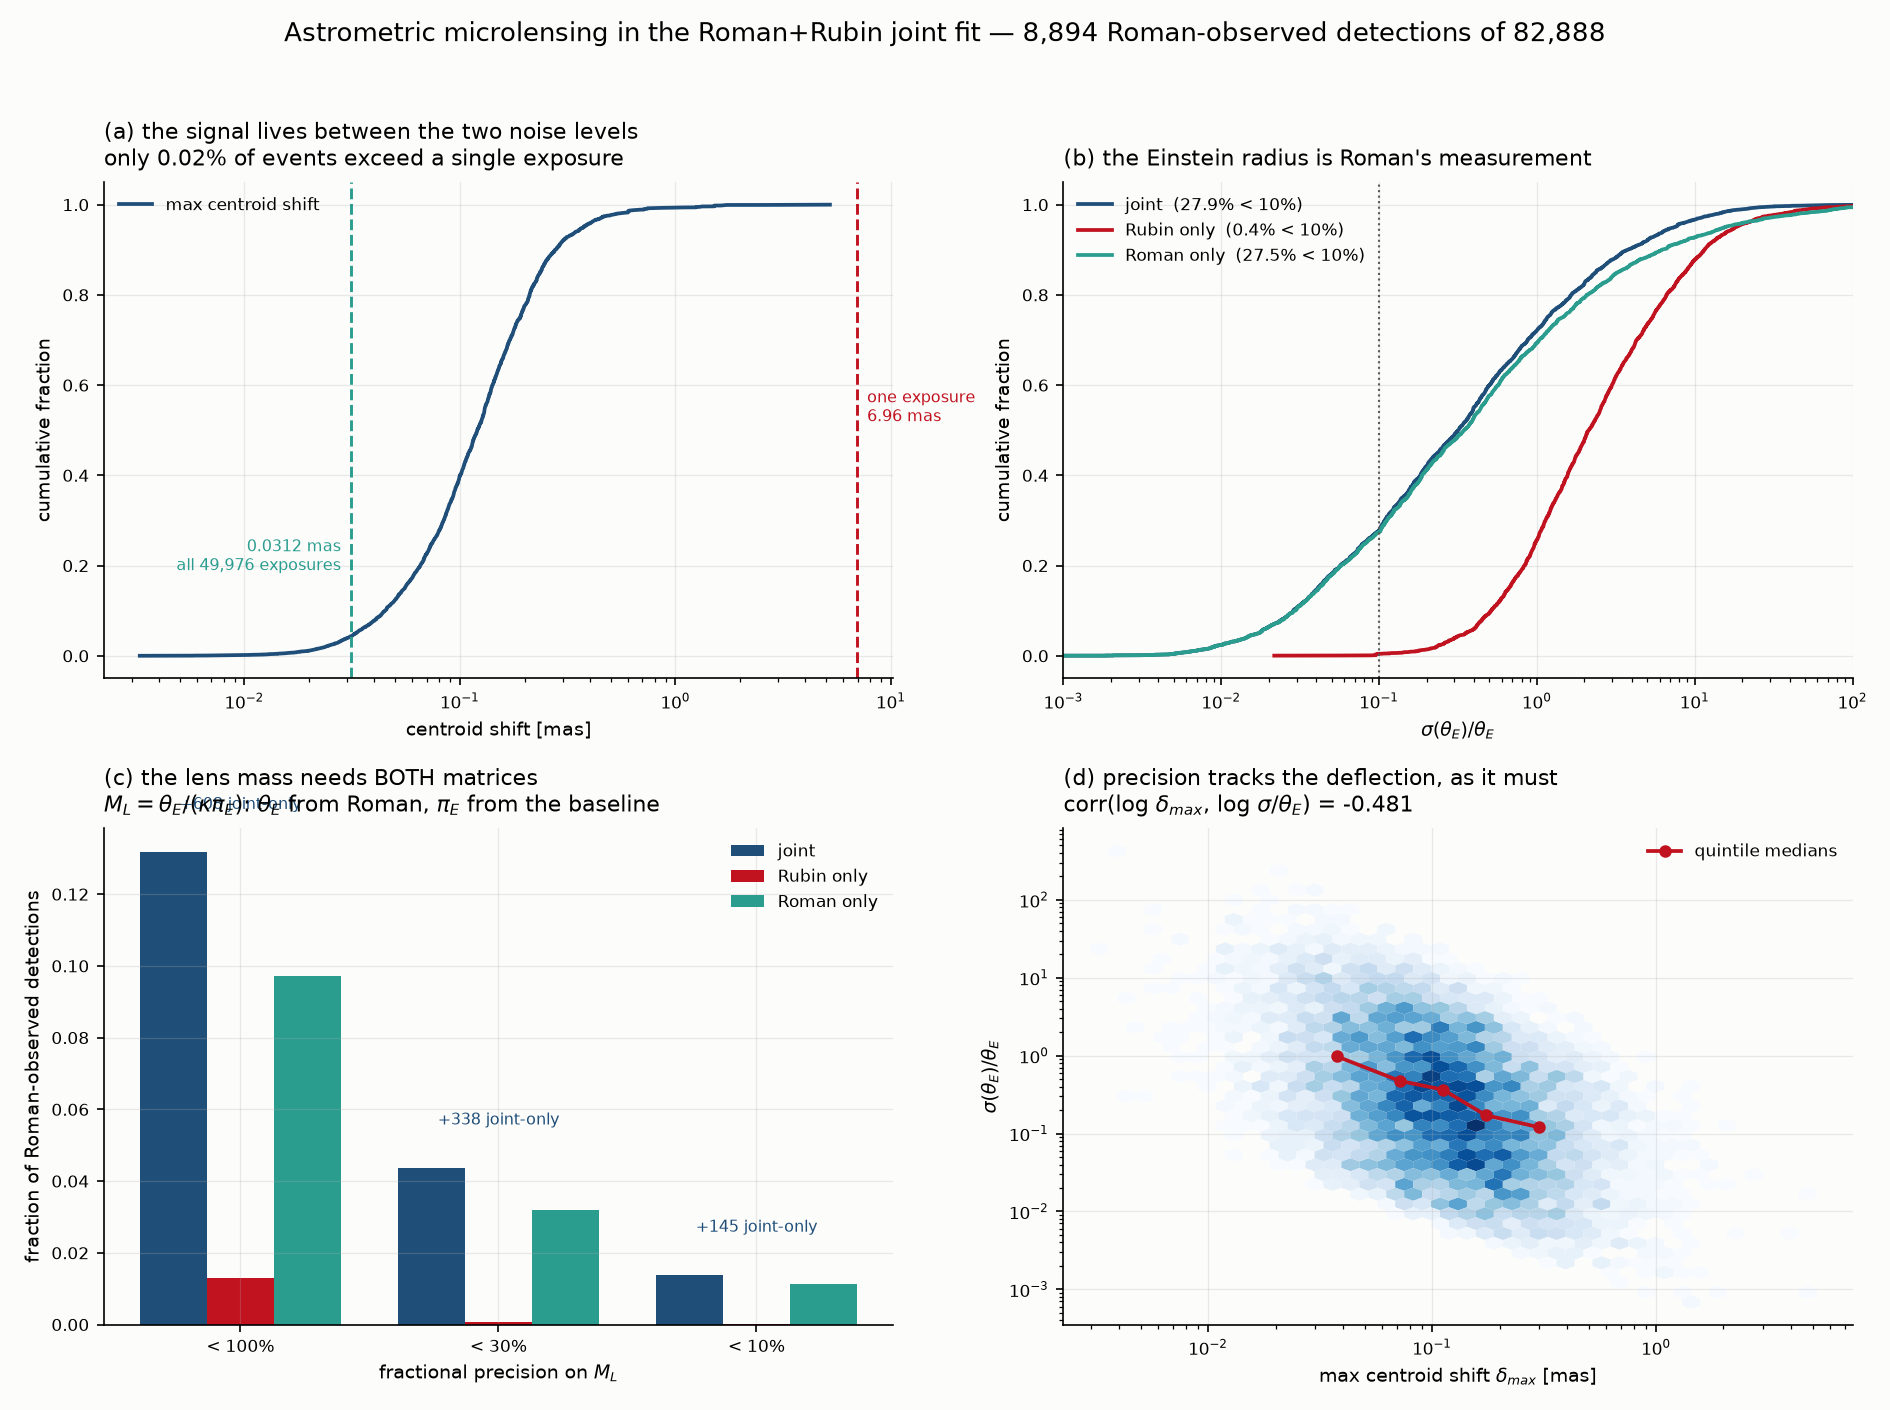
\includegraphics[width=\linewidth]{h5_astrometry_summary}
		\caption{The four claims the astrometric result rests on, each with the check that makes it testable, post-fix bulge run: (a) where the signal sits relative to one exposure and to the stack; (b) which instrument measures $\theta_E$; (c) the lens mass; (d) precision improving as the deflection grows -- a flat panel would mean the astrometric matrix is not responding to the deflection at all.}
		\label{fig:h5sum}
	\end{figure}

	\textbf{$\theta_E$ is Roman's measurement.} Median fractional precision $\sigma(\theta_E)/\theta_E$ is $0.098$ for the joint fit, $0.099$ for Roman alone and $2.30$ for Rubin alone. The paired, event-by-event median of $\sigma_{\mathrm{joint}}/\sigma_{\mathrm{Roman}}$ is $0.9988$ (pre-fix $0.977$): Rubin adds a tenth of a per cent. Against Rubin alone the joint fit is $31\times$ better.

	\textbf{The lens mass is still the quantity that needs both telescopes.} $M_L=\theta_E/(\kappa\pi_E)$ takes $\theta_E$ from Roman's astrometry and $\pi_E$ from the photometric baseline. Counting Roman-observed detections whose mass the joint fit measures to a given precision and \emph{neither survey alone} does: $494$ at better than $100\%$, $319$ at better than $30\%$ and $\mathbf{143}$ at better than $10\%$ (pre-fix $608$, $338$, $145$). As weighted shares of the footprint population they are $1.8\%$, $0.82\%$ and $0.22\%$. Counting instead events where a mass merely \emph{exists} returns none exclusive to the joint fit, because Rubin's matrix inverts for almost all of them -- with a median fractional mass error of $206$, i.e.\ $20{,}600\%$. An inverted matrix is not a measured mass.

	\subsection{Satellite parallax: Roman at L2 against Roman at Earth}
	\label{subsec:satpar}

	Roman observes from L2 and Rubin from the ground, so the two see the source along slightly different lines of sight, and the microlens parallax acquires a \emph{simultaneous} baseline beside the time-evolving annual one. The observable is the observer separation in Einstein radii, $\Delta u_{\mathrm{sat}} = \pi_E D_\perp/\mathrm{AU}$, a few thousandths; a large gain would be surprising, and whether a small one is measurable depends on cadence, errors and the correlation structure of the Fisher matrix.

	\paragraph{The experiment must be paired, and the obvious design does not work.} Two runs differing only in the offset diverge from the first sightline where the effect is non-zero, because moving the observer changes which events are detectable and the random stream is shared across the scan: measured, they agree exactly for $1{,}740{,}091$ events and part company at precisely the first field inside Roman's footprint. An unpaired comparison of the two detected populations was tried and rejected by its own control, reporting the satellite making the \emph{timescale} $15\%$ worse -- impossible for matched events. The comparison is therefore made inside one run (Section~\ref{subsec:perepoch}): each detected event characterised twice, with and without the offset, events with no Roman epochs near the peak kept as a control on which the ratio must be exactly $1$.

	\begin{figure}[htbp]
		\centering
		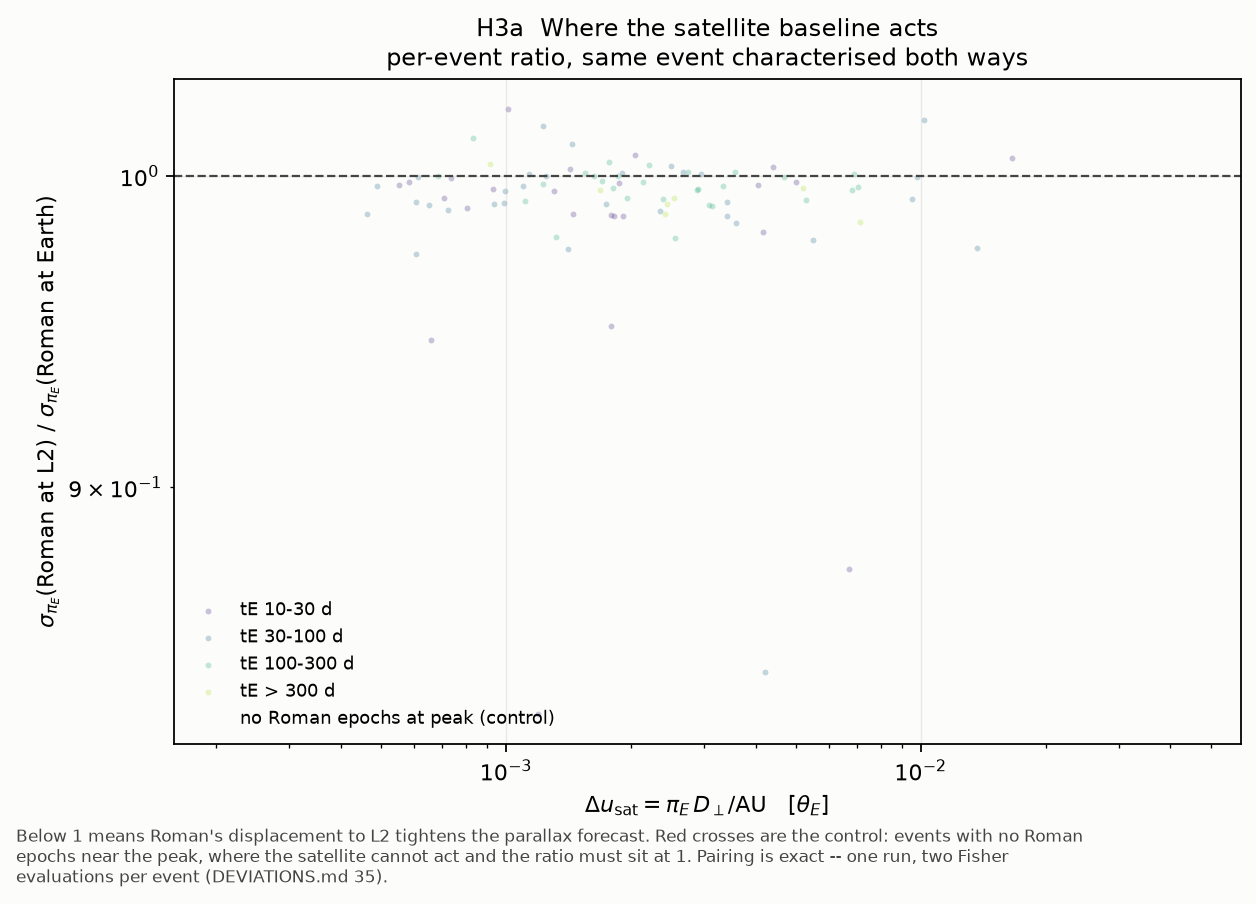
\includegraphics[width=\linewidth]{h3a_where}
		\caption{Per-event $\sigma_{\pi_E}$(Roman at L2)$/\sigma_{\pi_E}$(Roman at Earth) against the observer separation in Einstein radii, coloured by $t_E$; post-fix bulge run, the whole footprint. Below $1$: the displacement to L2 tightens the parallax forecast.}
		\label{fig:h3a}
	\end{figure}

	\textbf{Satellite parallax improves $\sigma(\pi_E)$ by under one per cent, and the improvement is real.} Over the $10{,}806$ Roman-covered events of the full footprint, weighted to $N_{\rm eff}=3{,}521$, the median ratio is $0.9911$ (quartiles $0.9878$--$0.9948$); $86.8\%$ of non-tied events improve. The control returns a median of exactly $1.000000$ over $72{,}082$ events, $95.1\%$ of them bit-exactly $1$. $40.7\%$ of covered events improve by more than $1\%$ and $1.2\%$ by more than a factor two; the latter sit at a median $t_E$ of $5.3$~d and $u_0$ of $0.34$ -- short, fairly high-magnification events, where the light curve changes fast enough that a small difference in observer position shows. Elsewhere the observer move does what it must: $\sigma(\theta_E)$ median ratio $0.99986$ (the Einstein radius comes from the deflection amplitude, not a baseline), $\sigma(t_E)$ $0.9997$, and the two geometries' condition numbers agree to $0.3\%$. The lens mass inherits the parallax gain, median $0.9935$.

	These numbers replace two limitations of the earlier version: they cover the whole footprint (before: $528$ events on a contiguous quarter of it), and they are event-rate weighted, which the earlier paired file could not be because it lacked the lens distance and velocity; the file now carries them. The weighted and raw medians agree closely ($0.9911$ and $0.9922$).

	\paragraph{A validation gate that could not have worked.} An obvious check is to require the gain to grow with $\Delta u_{\mathrm{sat}}$. It tests nothing: $D_\perp$ is one observatory's orbit, nearly the same for every event, so $\Delta u_{\mathrm{sat}}$ is essentially $\pi_E$ times a constant ($\mathrm{corr}(\log\pi_E,\log\Delta u_{\mathrm{sat}})=+0.9985$ in the earlier sample), and the check tests a dependence on $\pi_E$. It is replaced by five checks that follow from the physics, all passed here: the control bit-exact, $\sigma(t_E)$ intact, $\sigma(\theta_E)$ untouched, comparable conditioning, and a sign test against the control's exact null. The number of Roman epochs near the peak shows no trend either: a simultaneous baseline is a geometric constraint, fixed once a few epochs see the source from both positions.

	\subsection{Two baselines, at the same scale}
	\label{subsec:twobaselines}

	The two effects are both described as ``combining Roman and Rubin'', and they are different physics: a \emph{temporal} baseline -- one observatory's gaps filled by another's year-round cadence -- and a \emph{spatial} one -- two observatories $0.01$~AU apart. Figure~\ref{fig:h3c} puts them on one axis, both as weighted medians over the events each applies to.

	\begin{figure}[htbp]
		\centering
		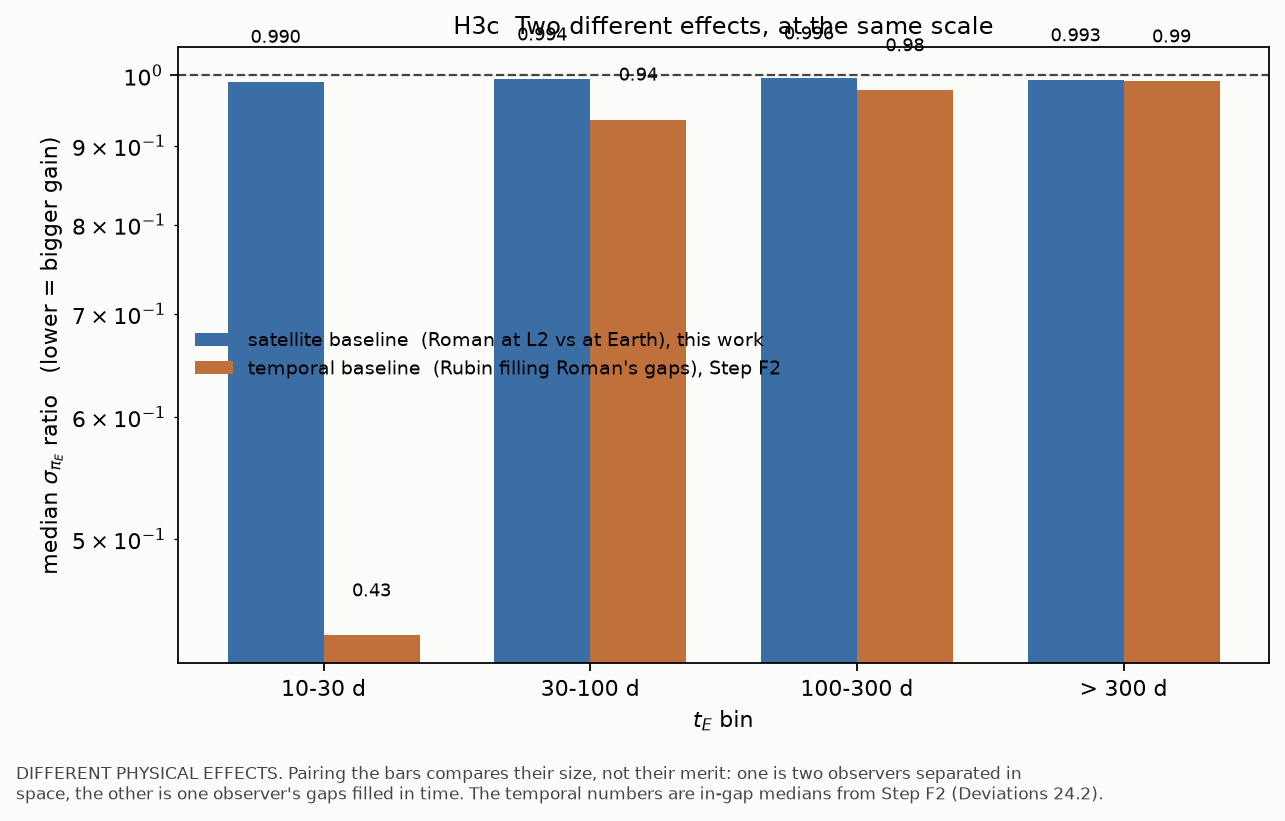
\includegraphics[width=0.85\linewidth]{h3c_honest}
		\caption{Median improvement in $\sigma(\pi_E)$ for each effect, per $t_E$ bin, event-rate weighted. Blue: Roman at L2 against Roman at Earth, the same event twice. Orange: the joint fit against Roman alone, for footprint events peaking in a season gap. Pairing the bars compares their size, not their merit.}
		\label{fig:h3c}
	\end{figure}

	The pre-fix version of this paper found the temporal baseline worth $\sim$$50$ times the spatial one for short events and concluded that the case for observing with both facilities rests on Rubin covering Roman's gaps, not on the L2 separation. \textbf{Corrected, the two are the same size}: for $10$--$30$~d events, pooled over the gap, $1.6\%$ against $0.9\%$; for longer events the satellite's sub-per-cent gain is the larger, the temporal one being nil. Both are small when pooled, and each is large only in its own corner -- the temporal gain for short events deep inside a gap (a factor $13$ beyond $45$~d), the spatial gain for a per-cent of short, high-magnification events (a factor two or more).

	\subsection{Black holes and neutron stars}
	\label{subsec:compact}

	The two compact-object runs (Section~\ref{subsec:populations}) were analysed the same way; the full account is the report \texttt{Report/postfix/}, and the yields are in Section~\ref{sec:yields}. Four results matter here.

	\begin{figure}[htbp]
		\centering
		\includegraphics[width=\linewidth]{p6_synergy}
		\caption{Compact-object runs. (a) Weighted share of detected events by who detects them. (b) Median joint/single-survey $\sigma(t_E)$ ratio against $t_E$, over events characterised by both surveys.}
		\label{fig:p6synergy}
	\end{figure}

	\emph{Detection share.} Roman alone detects $21.5\%$ of black-hole and $26.3\%$ of neutron-star events (pre-fix $5.3$ and $6.3\%$), Rubin alone $73\%$ and $70\%$, both $5.6\%$ and $3.9\%$. \emph{The joint gain.} On events both surveys characterise ($23{,}961$ and $18{,}895$), the median joint/Roman ratio is $0.997$--$0.999$ for $t_E$, $\pi_E$ and $\theta_E$ in both populations, flat across four decades of $t_E$ (Figure~\ref{fig:p6synergy}b), while joint/Rubin is $0.008$--$0.041$. Rubin's decade adds nothing measurable to Roman's ten seasons for these long events, because at the footprint's extinction its sources are several magnitudes fainter than Roman's. \emph{Astrometry.} The centroid shift exceeds Roman's $1.1$~mas floor for $90.4\%$ of black-hole detections and $0.58\%$ of neutron-star ones, unchanged by the fix. Satellite parallax is worthless for both (median gain exactly $1$; fewer than $0.2\%$ gain $10\%$), since their events last months to years. \emph{Image resolution} (Section~\ref{subsec:perepoch}): Roman resolves the two images of $65.5\%$ of its black-hole detections at $\mathcal{D}=5$, $30.9\%$ at $\mathcal{D}=20$ and $0.68\%$ at its PSF FWHM; for neutron stars $14.9\%$, $0.35\%$ and $0.001\%$. The two orders of magnitude between criteria outweigh every other effect.

	\paragraph{Against \cite{SajadianSahu2023}.} Their forecast for isolated black holes with Roman is the natural comparison, and it needs alignment first: their $F_1 = 0.019$ is the same kind of quantity as our $F$; their $\mathrm{d}N/\mathrm{d}M\propto M^{-1}$ row matches our log-uniform function; and our draws are re-weighted to $3$--$50\,M_\odot$ against their $2$--$50$ (Section~\ref{sec:yields}). Then Roman detects $464$ black holes in its footprint over ten seasons, $31.5$ per deg$^2$ per season against their $7.2$ -- a factor $4.4$, part of which is the survey design (the final GBTDS fills the $2.3$-year gap their forecast was built around \cite{ROTAC2025}) and part their stricter detection cut. On their denominator, the fraction of detections characterised to $10\%$ is, ours against theirs: $\theta_E$ $88.8$ vs $99.2\%$; $t_E$ $26.0$ vs $67.0\%$; $\pi_E$ $10.0$ vs $30.0\%$; $M_L$ $9.3$ vs $29.8\%$. The extinction fix closed most of the astrometric shortfall ($\theta_E$ was $68.6\%$) but little of the photometric one, so the parallax deficit has another cause (Section~\ref{sec:openitems}).


	\section{Open items}
	\label{sec:openitems}

	Stated plainly, because this document is meant to be usable by someone deciding whether to build on it. They are ordered by how much they would move the numbers above.

	\begin{itemize}
		\item \textbf{Roman's $1.1$~mas centroiding floor is treated as independent between exposures, and it may not be.} This is the dominant caveat on every $\theta_E$ and lens-mass number here. The Fisher sum gives each epoch an independent weight, so $N\approx5\times10^{4}$ exposures buy a factor $\sqrt{N}\approx224$ and take the median $2.75$~mas per-exposure precision of these sources to $0.012$~mas. But the floor is documented as a \emph{centroiding systematic} -- $1\%$ of the pixel, which is why it does not improve for brighter stars -- and a systematic of that kind is exactly the sort of error that correlates between exposures, through the PSF model, the distortion solution or the reference frame. In the fully correlated limit the effective precision approaches the full per-exposure value, the median signal sits nearly two orders of magnitude below the noise, and $\theta_E$ would not be measurable at all. Note that some averaging is demonstrably real: the $\sim$$0.1$~mas figure quoted for $\sim$$100$ stacked exposures \cite{Sanderson2019WFIRSTastrometry} is almost exactly $1.1/\sqrt{100}$, implying the floor is close to fully white over $100$ exposures. Whether that continues for another factor of $500$ in $N$ is the open question, and neither source addresses it. The fix is a two-component error model, $\sigma_{\mathrm{eff}}^2 = \sigma_{\mathrm{white}}^2/N + \sigma_{\mathrm{corr}}^2$, with the split taken from the Roman astrometry literature rather than assumed; inventing a split would be worse than naming the assumption.

		\item \textbf{Roman's photometric error model is a placeholder.} It is a nearest-neighbour lookup in a tabulated magnitude--error curve, not an interpolation, and the provenance of that table has not been verified against the F146 noise model of \cite{Wilson2023GBTDS}. Every photometric forecast for Roman inherits whatever that table is.

		\item \textbf{The modelled centroid is the source's, undiluted by blending.} A real measurement sees the centroid of everything in the aperture, so an unlensed blend drags the observed shift down by roughly the source-flux fraction. The photon-noise half of blending \emph{is} modelled -- the astrometric error is evaluated at the blended magnitude -- but the dilution half is not. For Roman the simplification is close to exact: at a $0.105''$ PSF the median source-flux fraction is $1.0$ and only $\sim$$11\%$ of events have any blend at all. For Rubin, at a median blend fraction of $0.45$, it is not; Rubin's astrometry carries no weight in any result here, but this is the reason not to start quoting it.

		\item \textbf{Roman's halo orbit about L2 is not modelled.} The mean offset is used. The halo orbit adds a periodic $10^{5}$--$10^{6}$~km wobble on an effect already of order $10^{-3}$, so it is a fractional correction to a small number -- but it is a correction in exactly the quantity Section~\ref{subsec:satpar} measures.

		\item \textbf{The adopted GBTDS footprint is Penny et al.'s, and the footprint has since changed.} Rubin's wide field also sees more of the bulge than the adopted region, which matters for blending as well as for coverage.

		\item \textbf{The per-sightline stopping criterion is weak in its third floor}, requiring only two well-conditioned Fisher matrices, so a field can complete with very few characterisable events and a noisy per-field precision estimate (Section~\ref{sec:fisher_caveats}).

		\item \textbf{The sample is stratified in sky position only.} Stratifying in $t_E$ as well would sharpen the short-$t_E$ bins, which is where the gap-filling effect lives and where the bins are thinnest.

		\item \textbf{The Rubin-alone branch has not been validated against an independent published forecast.} The natural comparison is \cite{Abrams2025MicrolensingRubin}, and it must reweight to their sampling first, or the difference in selection will look like a bug in this code.
			\item \textbf{The model's event rate is too flat in Galactic latitude.} Against OGLE-IV \cite{Mroz2019OGLEIV} the model over-produces the rate per star by $38\%$ at $b=-5.1^\circ$ and under-produces it by up to $50\%$ near the plane, crossing unity at $b\approx-2.3^\circ$ (Section~\ref{sec:yields}). Full-scan yields carry a systematic of a few tens of per cent, and the footprint sits where the model is $25$--$40\%$ low, so footprint yields are if anything understated. The cause -- the density normalisation, the source counts, or the extinction that sets which sources enter an $I<21$ sample -- is not known.

		\item \textbf{Roman's detection rate exceeds Penny et al.'s upper bracket.} $80.4$ events per deg$^2$ per day against their $63.8$ at $|u_0|<3$ \cite{penny2019predictions}. Known differences (ten seasons including four low-cadence ones; a different detection criterion) push in this direction but have not been shown to account for a factor $1.26$.

		\item \textbf{Roman's forecast parallax precision is $\sim\!3\times$ worse than \cite{SajadianSahu2023}'s}, on matched assumptions, and the extinction law is now ruled out as the main cause. Candidates: whether the photometric and astrometric $\pi_E$ information are combined as they should be, and the long parallax baseline of the gap observations they add by hand.

		\item \textbf{The table's $t_0$ is not the observed peak} (Section~\ref{subsec:samples}): it is referenced to the Earth's position at $t=0$, and the columns derived from it -- which season the peak falls in, its distance to a season edge, the epochs near the peak -- inherit the offset. Every gap-filling statistic is binned on them. For most events the offset is days.

		\item \textbf{One detection-test anomaly} in the $85{,}061$ bulge detections: a single-survey test passed and the joint test did not, which the construction of Section~\ref{subsec:detclass} should forbid. The flag is made monotone downstream, so no table is wrong; the event has not yet been inspected.

		\item \textbf{The black-hole remnant masses of the ordinary-lens population are a single slope}, $M_{\rm BH} = 0.24\,M_i$. Real remnant masses depend on metallicity and mass loss in ways no slope captures, and these lenses populate the long-$t_E$ tail the gap-filling and parallax results depend on. The neutron-star population's single Gaussian likewise understates a probable high-mass recycled component.

		\item \textbf{The F146 extinction scatter and several F146 constants are placeholders}: the per-band extinction scatter $\sigma_i$ uses a K-band value for F146 (Section~\ref{subsec:reddening}), and the F146 PSF width in \texttt{Bulge.h} is an ELT-scale value (Table~\ref{tab:gbtds_design}).

\end{itemize}

	\bibliographystyle{ieeetr}
	\bibliography{refs}
	% ---------------------------------------------------------------------------------------------
% DRAFT appendix: finite-difference step-size convergence test (refactor plan Step C3).
%
% \input{} at the end of whitepaper.tex.
%
% Figure dependency: c3_step_sweep.png, produced by
%     ./fishertest --sweep > c3_sweep.csv
%     python tests/c3_step_sweep.py c3_sweep.csv -o c3_step_sweep.png
% Copy it into Whitepaper/ before compiling.
% ---------------------------------------------------------------------------------------------

\appendix

\section{Finite-difference step sizes and the convergence of the Fisher forecast}
\label{app:stepsize}

Every derivative in Section~\ref{sec:fisher} is computed numerically, by perturbing a parameter
and re-evaluating the model. The forecast therefore inherits whatever error that approximation
carries, and the size of the perturbation is a free choice that nothing in the physics fixes.
Because the precision gains this paper reports are in places at the few-per-cent level, a
differencing error at that same scale would be indistinguishable from the signal. This appendix
establishes that it is not.

\subsection{Why a step size has a correct value at all}
\label{app:stepsize_theory}

A central-difference estimate of a derivative,
\[
\frac{\partial m}{\partial\theta} \simeq \frac{m(\theta+h) - m(\theta-h)}{2h},
\]
carries two errors that pull in opposite directions. Expanding in a Taylor series, the neglected
terms give a \emph{truncation} error of order $h^2 m'''$, which grows as the step grows: the
secant through two widely separated points stops matching the tangent. Working against it,
evaluating $m$ in finite precision gives a \emph{round-off} error of order $\epsilon |m| / h$,
which grows as the step shrinks: subtracting two nearly equal numbers cancels their leading
significant digits, and dividing by a small $h$ amplifies what remains. Their sum is U-shaped in
$h$, with a broad flat minimum -- a plateau -- between the two regimes. A trustworthy step lies in
the middle of that plateau, and the plateau's existence, not merely the value chosen from it, is
what has to be demonstrated.

For a Fisher forecast the consequence is sharper than a general loss of accuracy, because the
error does not distribute itself evenly across the matrix. This is developed in
Section~\ref{app:stepsize_eigen}.

\subsection{The measurement}
\label{app:stepsize_measure}

The step for each parameter was swept over twelve decades while all other steps were held at their
default, and the recovered $\sigma$ recorded. The sweep uses a synthetic-event fixture rather than
the full Monte Carlo: seven events spanning $t_E$ from $5$ to $900$~d, each in two versions --
peaking inside a Roman high-cadence season and peaking in a Roman gap -- evaluated separately for
the joint, Rubin-only and Roman-only partitions of Section~\ref{subsec:partition}. Using a fixture is
what makes the test affordable (seconds rather than the hours needed to accumulate a comparable
number of Fisher-scored events from the Monte Carlo), and it isolates the numerical question from
the population statistics.

Two of the nine photometric parameters serve as controls. The model magnitude depends on the
baseline magnitudes $m_{b,0}$ and $m_{b,1}$ linearly and with unit slope, so their finite
difference is exact at any step and their curves must be perfectly flat. Any structure there would
indicate a fault in the sweep machinery rather than in the physics. Both are flat to machine
precision across all twelve decades.

Figure~\ref{fig:stepsweep} shows the result. Both walls of the expected U are visible, bracketing a
plateau roughly seven decades wide, across which $\sigma$ is stable to better than $0.1\%$ for
every parameter and every event.

\begin{figure}[htbp]
	\centering
	\includegraphics[width=\linewidth]{c3_step_sweep}
	\caption{Recovered parameter uncertainty $\sigma$ as a function of the finite-difference step,
	for each of the nine photometric parameters (panels), seven test events (colours) and three
	survey partitions (line styles). The step is plotted relative to the adopted value, so the
	adopted step is the vertical line at $1$ and the shaded band marks the plateau. Curves are
	normalised to the adopted step, so a converged parameter is a flat line at unity. The collapse
	at small steps is round-off; the collapse at large steps is truncation. The two baseline-
	magnitude panels ($m_{b,0}$, $m_{b,1}$) are controls: the model is exactly linear in these, so
	their flatness across the full range validates the sweep itself. Note that both failure modes
	drive $\sigma$ \emph{downward} -- they manufacture apparent information rather than destroying
	it, which is why neither announces itself as an obviously broken result.}
	\label{fig:stepsweep}
\end{figure}

\subsection{The steps adopted here}
\label{app:stepsize_adopted}

The simulation inherited its step sizes from a legacy codebase written for a different
science case, where they were expressed as fixed fractions of each parameter: $0.151$ for $u_0$
(against a typical $u_0 \sim 0.3$), $0.255\,t_E$ for both $t_E$ and $t_0$, $0.251\,\pi_E$ for
$\pi_E$, and $3^\circ$ for the trajectory angle $\xi$. Figure~\ref{fig:stepsweep} places all of
these far up the truncation branch: they are approximately four orders of magnitude larger than
the plateau. Every step is therefore scaled by a single factor of $10^{-4}$, which places all nine
in the middle of the plateau simultaneously. A factor of $10^{-5}$ reproduces every $\sigma$ to
better than $0.3\%$, so the result is not sensitive to where in the plateau the step is taken.

Table~\ref{tab:stepbias} gives the cost of the original choice. The entries are the factor by
which the legacy step \emph{understated} the recovered uncertainty, which is the quantity that
matters: in every case the error is in the optimistic direction.

\begin{table}[htbp]
	\centering
	\caption{Factor by which the legacy finite-difference steps understated the forecast
	uncertainty, $\sigma_{\mathrm{converged}} / \sigma_{\mathrm{legacy}}$, over all test events and
	survey partitions. A value of $1.00$ means the legacy step was already adequate for that
	parameter. The two baseline magnitudes are the linear controls.}
	\label{tab:stepbias}
	\begin{tabular}{lrr}
		\toprule
		Parameter & Median & Worst case \\
		\midrule
		$u_0$        & 21.7 & 7643 \\
		$t_0$        &  6.0 & 10388 \\
		$t_E$        &  1.45 &  26.1 \\
		$\pi_E$      &  1.00 & 219.8 \\
		$\xi$        &  1.00 &  45.6 \\
		$f_{b,0}$, $f_{b,1}$ & 1.00 & 1.01 \\
		$m_{b,0}$, $m_{b,1}$ (control) & 1.00 & 1.00 \\
		\bottomrule
	\end{tabular}
\end{table}

The median and worst-case columns differ by orders of magnitude because the damage is
concentrated on the events whose Fisher matrices are closest to degenerate -- short events, and
events with sparse coverage. For $\pi_E$ and $\xi$ the median is unity: on a typical
well-sampled event the legacy step was harmless, and the failure appears only where the matrix is
already nearly singular. This is precisely the population that the joint-fit science case is about.

\subsection{Where the error goes: the eigenstructure of the Fisher matrix}
\label{app:stepsize_eigen}

That the errors concentrate on near-degenerate events is not a coincidence, and it explains why
the effect is larger than the per-parameter percentages suggest.

The Fisher matrix is assembled in physical units, so its entries carry units of
$1/(\theta_j\theta_k)$ and span many orders of magnitude before any physics enters --
$t_E$ is measured in days ($\sim 30$), $u_0$ is dimensionless ($\sim 0.3$), $\xi$ is in radians.
Normalising by $\tilde{F} = D F D$ with $D = \mathrm{diag}(1/\sqrt{F_{ii}})$ removes this: the
diagonal becomes unity, every off-diagonal entry becomes a correlation coefficient, and the
inverse is recovered exactly as $F^{-1} = D\tilde{F}^{-1}D$. Whatever ill-conditioning survives in
$\tilde{F}$ is a statement about the data, not about the choice of units.

Diagonalising $\tilde{F}$ rotates onto parameter \emph{combinations} that are measured
independently, with eigenvalue $\lambda_k$ the information carried about combination $k$ and
$\lambda_{\max}/\lambda_{\min}$ the condition number. A large condition number is usually not a
numerical inconvenience but a physical fact: some combination of parameters genuinely cannot be
recovered from that light curve, and the eigenvector belonging to $\lambda_{\min}$ names it.
For a short event observed only sparsely, that direction is the familiar $u_0$--$\pi_E$
degeneracy; for an event with poorly sampled wings it is the $t_E$--$f_b$ degeneracy between a
longer, more blended event and a shorter, less blended one.

Comparing the normalised spectrum of a $5$-day event at the legacy and converged steps makes the
mechanism explicit:

\begin{center}
\begin{tabular}{lcccc}
	\toprule
	& $\lambda_1 \ldots \lambda_6$ & $\lambda_7$ & $\lambda_8$ & $\lambda_9$ \\
	\midrule
	Legacy steps    & $3.30, 1.83, 1.30, 1.19, 0.712, 0.532$ & $7.5\times10^{-2}$ & $6.1\times10^{-2}$ & $5.3\times10^{-3}$ \\
	Converged steps & $3.42, 1.89, 1.30, 1.16, 0.711, 0.513$ & $7.8\times10^{-3}$ & $8.7\times10^{-7}$ & $2.3\times10^{-10}$ \\
	\bottomrule
\end{tabular}
\end{center}

\noindent The six best-constrained directions are essentially unchanged. The entire discrepancy
sits in the three flattest ones, where the smallest eigenvalue is inflated by a factor of
$\sim\!4\times10^{7}$ and the condition number consequently reads $6.2\times10^{2}$ instead of its
true $1.5\times10^{10}$. Since $\tilde{F}$ has unit diagonal its trace is fixed at the dimension,
so no information was created: it was redistributed out of the well-constrained directions into
the degenerate ones. Physically, truncation error was papering over real parameter degeneracies --
the legacy configuration reported a sub-per-cent parallax measurement for an event far too short
to exhibit annual parallax at all.

This is the reason the convergence test is reported here rather than being treated as an internal
numerical detail. An unconverged derivative in a Fisher forecast does not present as scatter; it
presents as a confident, well-conditioned, and entirely spurious measurement of exactly those
parameter combinations the data cannot constrain.

\subsection{Effect on the results of this paper}
\label{app:stepsize_impact}

Two consequences, of very different weight.

First, absolute parameter uncertainties are affected, and every $\sigma$ quoted here is computed
with the converged steps. Forecasts made with the legacy configuration were optimistic, severely so
for short-$t_E$ events.

Second -- and this is what matters for the paper's claims -- the \emph{relative} results are
robust. Because the joint, Rubin-only and Roman-only matrices are accumulated from the same
simulated event with the same random draws, the comparison between them is paired, and a common
multiplicative error in the derivatives largely cancels in the per-event ratio. Table
\ref{tab:stepratio} shows the headline quantity, the ratio of the joint-fit uncertainty on $t_E$ to
the better of the two single-survey fits, computed either side of the correction.

\begin{table}[htbp]
	\centering
	\caption{Ratio $\sigma_{t_E}^{\mathrm{joint}} / \min(\sigma_{t_E}^{\mathrm{Rubin}},
	\sigma_{t_E}^{\mathrm{Roman}})$ for each test event, computed with the legacy and the converged
	finite-difference steps. Values below unity indicate the joint fit outperforms either survey
	alone. Events labelled ``gap'' peak between Roman observing seasons.}
	\label{tab:stepratio}
	\begin{tabular}{lrr}
		\toprule
		Event & Legacy steps & Converged steps \\
		\midrule
		$t_E = 5$~d, in season    & 0.9995 & 0.9981 \\
		$t_E = 5$~d, in gap       & 1.0000 & 1.0000 \\
		$t_E = 25$~d, in season   & 0.9980 & 0.9902 \\
		$t_E = 25$~d, in gap      & 1.0000 & 1.0000 \\
		$t_E = 100$~d, in season  & 0.9935 & 0.9717 \\
		$t_E = 100$~d, in gap     & 0.9788 & 0.9827 \\
		$t_E = 900$~d             & 0.7588 & 0.7951 \\
		\bottomrule
	\end{tabular}
\end{table}

The ordering is preserved and the magnitudes shift by at most a few per cent, with the joint-fit
advantage slightly larger after correction in most cases. The two events where it is smaller are
instructive: in both, the correction falls more heavily on the survey playing the supporting role
than on the one that dominates the fit. For the $100$-day gap event, Roman is the weaker partner --
it barely covers the peak -- and its $\sigma_{t_E}$ inflates by a factor $2.14$ against Rubin's
$1.28$. For the $900$-day event, Rubin's contribution is specifically the parallax channel, its
continuous coverage sampling the annual signal across Roman's seasonal gaps, and its
$\sigma_{\pi_E}$ inflates by $2.18$ against Roman's $1.10$. This mechanism is inferred from seven
constructed events and should be regarded as a plausible reading rather than an established
property.

\subsection{A note on the differencing scheme}
\label{app:stepsize_stencil}

The sweep also settled a question left open in Section~\ref{sec:fisher}: why $t_E$ and $\pi_E$ were
differenced with both evaluations on the same side of the parameter value, rather than
symmetrically. The pattern applies to exactly the parameters constrained to remain positive, which
suggests the intent was to avoid evaluating the model at an unphysical value. That is not a real
constraint at these step sizes, and the cost is significant: averaging two one-sided differences
gives $m'(\theta) + \tfrac{3}{8}m''(\theta)h + \mathcal{O}(h^2)$, a first-order and biased estimate,
against the second-order symmetric form. Verified on a smooth test function, the one-sided scheme
carries $\approx\!22\times$ the error at equal step and improves by only one decade per decade of
step reduction, against two. Both parameters now use the symmetric form. At the converged step the
numerical difference is immaterial, since the bias term scales with $h$; the change removes a
latent sensitivity rather than altering a result.

The corresponding astrometric derivatives ($\theta_E$ and $\pi_E$ in the astrometric matrix) retain
the one-sided scheme, and their steps have not been swept. This is deliberate: the astrometric
forecast also depends on the unresolved question of Roman's F146 astrometric error model noted in
Section~\ref{sec:fisher_caveats}, so its absolute uncertainties are not yet quantitative regardless
of the differencing scheme, and correcting one of two unverified inputs in isolation would not be
checkable. Both should be addressed together.

	
\end{document}